% Use only LaTeX2e, calling the article.cls class and 12-point type.
%DIF LATEXDIFF DIFFERENCE FILE



\documentclass[12pt]{article}

% Users of the {thebibliography} environment or BibTeX should use the
% scicite.sty package, downloadable from *Science* at
% http://www.sciencemag.org/authors/preparing-manuscripts-using-latex
% This package should properly format in-text
% reference calls and reference-list numbers.

\usepackage{scicite}

\usepackage{times}

% Packages I manually added
\usepackage{graphicx}
\usepackage{placeins}
\usepackage{float}
\usepackage{amsmath}
\usepackage{hyperref}
\usepackage{pdflscape}



% The preamble here sets up a lot of new/revised commands and
% environments.  It's annoying, but please do *not* try to strip these
% out into a separate .sty file (which could lead to the loss of some
% information when we convert the file to other formats).  Instead, keep
% them in the preamble of your main LaTeX source file.


% The following parameters seem to provide a reasonable page setup.

\topmargin 0.0cm
\oddsidemargin 0.2cm
\textwidth 16cm
\textheight 21cm
\footskip 1.0cm


%The next command sets up an environment for the abstract to your paper.

\newenvironment{sciabstract}{%
\begin{quote} \bf}
{\end{quote}}



% Include your paper's title here

\title{Fishery Markets and Large-Scale Marine Conservation}


% Place the author information here.  Please hand-code the contact
% information and notecalls; do *not* use \footnote commands.  Let the
% author contact information appear immediately below the author names
% as shown.  We would also prefer that you don't change the type-size
% settings shown here.

\author{Juan CarlosVillase\~{n}or-Derbez,$^{1\ast}$ John Lynham,$^{2}$ Christopher Costello$^{1}$\\
\\
\normalsize{$^{1}$Bren School of Environmental Science \& Management,}\\
\normalsize{University of California at Santa Barbara, Santa Barbara, CA}\\
\normalsize{$^{2}$Department of Economics, University of Hawaii at Manoa, Honolulu, HI}\\
\\
\normalsize{$^\ast$To whom correspondence should be addressed; E-mail: juancarlos@ucsb.edu.}
}

% Include the date command, but leave its argument blank.

\date{}



%%%%%%%%%%%%%%%%% END OF PREAMBLE %%%%%%%%%%%%%%%%
%DIF PREAMBLE EXTENSION ADDED BY LATEXDIFF
%DIF UNDERLINE PREAMBLE %DIF PREAMBLE
\RequirePackage[normalem]{ulem} %DIF PREAMBLE
\RequirePackage{color}\definecolor{RED}{rgb}{1,0,0}\definecolor{BLUE}{rgb}{0,0,1} %DIF PREAMBLE
\providecommand{\DIFaddtex}[1]{{\protect\color{blue}\uwave{#1}}} %DIF PREAMBLE
\providecommand{\DIFdeltex}[1]{{\protect\color{red}\sout{#1}}}                      %DIF PREAMBLE
%DIF SAFE PREAMBLE %DIF PREAMBLE
\providecommand{\DIFaddbegin}{} %DIF PREAMBLE
\providecommand{\DIFaddend}{} %DIF PREAMBLE
\providecommand{\DIFdelbegin}{} %DIF PREAMBLE
\providecommand{\DIFdelend}{} %DIF PREAMBLE
%DIF FLOATSAFE PREAMBLE %DIF PREAMBLE
\providecommand{\DIFaddFL}[1]{\DIFadd{#1}} %DIF PREAMBLE
\providecommand{\DIFdelFL}[1]{\DIFdel{#1}} %DIF PREAMBLE
\providecommand{\DIFaddbeginFL}{} %DIF PREAMBLE
\providecommand{\DIFaddendFL}{} %DIF PREAMBLE
\providecommand{\DIFdelbeginFL}{} %DIF PREAMBLE
\providecommand{\DIFdelendFL}{} %DIF PREAMBLE
%DIF HYPERREF PREAMBLE %DIF PREAMBLE
\providecommand{\DIFadd}[1]{\texorpdfstring{\DIFaddtex{#1}}{#1}} %DIF PREAMBLE
\providecommand{\DIFdel}[1]{\texorpdfstring{\DIFdeltex{#1}}{}} %DIF PREAMBLE
\newcommand{\DIFscaledelfig}{0.5}
%DIF HIGHLIGHTGRAPHICS PREAMBLE %DIF PREAMBLE
\RequirePackage{settobox} %DIF PREAMBLE
\RequirePackage{letltxmacro} %DIF PREAMBLE
\newsavebox{\DIFdelgraphicsbox} %DIF PREAMBLE
\newlength{\DIFdelgraphicswidth} %DIF PREAMBLE
\newlength{\DIFdelgraphicsheight} %DIF PREAMBLE
% store original definition of \includegraphics %DIF PREAMBLE
\LetLtxMacro{\DIFOincludegraphics}{\includegraphics} %DIF PREAMBLE
\newcommand{\DIFaddincludegraphics}[2][]{{\color{blue}\fbox{\DIFOincludegraphics[#1]{#2}}}} %DIF PREAMBLE
\newcommand{\DIFdelincludegraphics}[2][]{% %DIF PREAMBLE
\sbox{\DIFdelgraphicsbox}{\DIFOincludegraphics[#1]{#2}}% %DIF PREAMBLE
\settoboxwidth{\DIFdelgraphicswidth}{\DIFdelgraphicsbox} %DIF PREAMBLE
\settoboxtotalheight{\DIFdelgraphicsheight}{\DIFdelgraphicsbox} %DIF PREAMBLE
\scalebox{\DIFscaledelfig}{% %DIF PREAMBLE
\parbox[b]{\DIFdelgraphicswidth}{\usebox{\DIFdelgraphicsbox}\\[-\baselineskip] \rule{\DIFdelgraphicswidth}{0em}}\llap{\resizebox{\DIFdelgraphicswidth}{\DIFdelgraphicsheight}{% %DIF PREAMBLE
\setlength{\unitlength}{\DIFdelgraphicswidth}% %DIF PREAMBLE
\begin{picture}(1,1)% %DIF PREAMBLE
\thicklines\linethickness{2pt} %DIF PREAMBLE
{\color[rgb]{1,0,0}\put(0,0){\framebox(1,1){}}}% %DIF PREAMBLE
{\color[rgb]{1,0,0}\put(0,0){\line( 1,1){1}}}% %DIF PREAMBLE
{\color[rgb]{1,0,0}\put(0,1){\line(1,-1){1}}}% %DIF PREAMBLE
\end{picture}% %DIF PREAMBLE
}\hspace*{3pt}}} %DIF PREAMBLE
} %DIF PREAMBLE
\LetLtxMacro{\DIFOaddbegin}{\DIFaddbegin} %DIF PREAMBLE
\LetLtxMacro{\DIFOaddend}{\DIFaddend} %DIF PREAMBLE
\LetLtxMacro{\DIFOdelbegin}{\DIFdelbegin} %DIF PREAMBLE
\LetLtxMacro{\DIFOdelend}{\DIFdelend} %DIF PREAMBLE
\DeclareRobustCommand{\DIFaddbegin}{\DIFOaddbegin \let\includegraphics\DIFaddincludegraphics} %DIF PREAMBLE
\DeclareRobustCommand{\DIFaddend}{\DIFOaddend \let\includegraphics\DIFOincludegraphics} %DIF PREAMBLE
\DeclareRobustCommand{\DIFdelbegin}{\DIFOdelbegin \let\includegraphics\DIFdelincludegraphics} %DIF PREAMBLE
\DeclareRobustCommand{\DIFdelend}{\DIFOaddend \let\includegraphics\DIFOincludegraphics} %DIF PREAMBLE
\LetLtxMacro{\DIFOaddbeginFL}{\DIFaddbeginFL} %DIF PREAMBLE
\LetLtxMacro{\DIFOaddendFL}{\DIFaddendFL} %DIF PREAMBLE
\LetLtxMacro{\DIFOdelbeginFL}{\DIFdelbeginFL} %DIF PREAMBLE
\LetLtxMacro{\DIFOdelendFL}{\DIFdelendFL} %DIF PREAMBLE
\DeclareRobustCommand{\DIFaddbeginFL}{\DIFOaddbeginFL \let\includegraphics\DIFaddincludegraphics} %DIF PREAMBLE
\DeclareRobustCommand{\DIFaddendFL}{\DIFOaddendFL \let\includegraphics\DIFOincludegraphics} %DIF PREAMBLE
\DeclareRobustCommand{\DIFdelbeginFL}{\DIFOdelbeginFL \let\includegraphics\DIFdelincludegraphics} %DIF PREAMBLE
\DeclareRobustCommand{\DIFdelendFL}{\DIFOaddendFL \let\includegraphics\DIFOincludegraphics} %DIF PREAMBLE
%DIF END PREAMBLE EXTENSION ADDED BY LATEXDIFF

\begin{document}

% Double-space the manuscript.

\baselineskip24pt

% Make the title.

\maketitle



% Place your abstract within the special {sciabstract} environment.
\begin{sciabstract}
Will rights-based approaches to managing natural resources facilitate, or impede large-scale conservation? We study this question in the context of large-scale marine protected areas, and ask whether a country that commits to large-scale conservation is destined to suffer commensurate losses in fishery income.  Indeed, this is a question maritime nations all over the world face as they consider whether, and how, to comply with \DIFdelbegin \DIFdel{various }\DIFdelend international commitments to expand marine protection. We use a combination of spatial bioeconomic modeling, which accounts for fisheries markets such as the vessel-day trading scheme in the Pacific Ocean, and vessel-level empirical data on fishing behavior before and after MPA implementation, to assess how market design incentivizes, or penalizes conservation. The answer hinges critically on two design features of the rights-based fishery market. First, only if trading of harvest or vessel-days is allowed across countries can a conservation-minded country capture the economic spillover benefits of their conservation actions.  Instead, if trading is forbidden, countries are likely to suffer losses from conservation. Second, when rights are allocated between countries, the allocation must depend only on biological features, and not on economic factors such as a country's past effort or catch. Otherwise, the allocation process acts as a punishment to the conserving country. Overall, these results show that seemingly \DIFdelbegin \DIFdel{innocuous }\DIFdelend \DIFaddbegin \DIFadd{benign }\DIFaddend design features of a market can have indelible impacts on a country's willingness to engage in large-scale conservation; these results are confirmed with an empirical case study from the Phoenix Islands Protected Area, one of the world's largest marine reserves. With the right design features, large-scale protected areas such as the Phoenix Islands can be achieved at close to zero cost to the implementing country.
\end{sciabstract}

%%%%%%%%%%%%%%%%%%%%%%%%%%%%%%%%%%%%%%%%%%%%%%%%%%%%%%%%%%


%%%% Other titles %%%%%%%%%%%%
% Fishery markets enable marine conservation
% Designing environmental markets for marine conservation
% Large-scale marine conservation is enabled by market instruments
% Rights-based management to promote marine conservation


%%%%%%%%%%%%%%%%%%%%%%%%%%%%%%%%%

Recognizing a need to secure biodiversity, blue carbon, rare habitats, and other ecosystem services, various international bodies have committed to dramatically expand marine protection around the world. Currently only about 3\% of the world's ocean is strongly protected \cite{sala_2018}, and these commitments call for 10\%, 30\%, or even up to 50\% of the ocean to be off-limits to fishing. Fundamentally, to achieve these goals, huge swaths of sovereign nations' waters will have to be closed to fishing. What incentives might motivate a country to engage in such large-scale marine protection? Would any country rationally close 20\%, 50\%, or even 100\% of its waters to fishing if this meant losing all fishing revenue from within its borders? We show that a country's incentives for large-scale conservation hinge critically on an unsuspected culprit: the design of fishing rights.

We are motivated by a real-world institution called the Parties to the Nauru Agreement (PNA). Like an OPEC for tuna, the PNA is a nine-country coalition of Pacific Island states that collectively manages tuna fishing in its members' waters\cite{havice_2013,aqorau_2018}. These waters collectively account for 14.5 million km\textsuperscript{2} (an area four times larger than the continental United States), and over 60\% of skipjack tuna catch in the Western Central Pacific \cite{havice_2013}.

In addition to highly productive tuna fisheries, the PNA waters provide a wealth of other ecosystem benefits, hence the focus on large-scale conservation efforts in the region. The PNA member nations derive enormous benefits from leasing tuna fishing rights to foreign fleets, in some cases exceeding \DIFdelbegin \DIFdel{50\% }\DIFdelend \DIFaddbegin \DIFadd{half }\DIFaddend of a country's \DIFdelbegin \DIFdel{annual revenue}\DIFdelend \DIFaddbegin \DIFadd{GDP}\DIFaddend . A natural concern arises: even if the closure creates net benefits to the world, and perhaps even to tuna fisheries Pacific-wide, the economic loss to the conserving country could still be extremely large, and may prevent it from engaging in any meaningful conservation. Intuitively, then, it seems that a country's willingness to engage in large-scale conservation will depend crucially on whether it can successfully capture a sufficiently high fraction of the benefits that are derived from that conservation. We show how a rights-based fisheries market can be designed (if it is new) or modified (if it already exists) to ensure that the conserving country is rewarded, not punished, for large-scale conservation.

\DIFdelbegin \DIFdel{We }\DIFdelend \DIFaddbegin \DIFadd{To mirror the strategies and spatial connections among the nine PNA countries and the high seas, we }\DIFaddend develop a 10-patch spatial bioeconomic model\DIFdelbegin \DIFdel{of a fishery operating under a }\DIFdelend \DIFaddbegin \DIFadd{. The fishery in nine of the patches operates under a market-based system in which ``vessel days'' are capped, closely tracked, and may be traded across countries.  This }\DIFaddend vessel-day scheme (VDS) \DIFdelbegin \DIFdel{, and where conservation is being considered. A VDS is a type of rights-based management approach }\DIFdelend \DIFaddbegin \DIFadd{is acutally }\DIFaddend used by the PNA\DIFdelbegin \DIFdel{where }\DIFdelend \DIFaddbegin \DIFadd{; }\DIFaddend each country is given an allocation of vessel-days that can then be sold to fishing firms. A vessel-day \DIFdelbegin \DIFdel{for }\DIFdelend \DIFaddbegin \DIFadd{owned by }\DIFaddend country $i$ \DIFdelbegin \DIFdel{gives a firm the right to have one vesselfish in country }\DIFdelend \DIFaddbegin \DIFadd{entitles $i$ to lease that day to a fishing vessel, entitling it to fish in }\DIFaddend $i$'s EEZ for \DIFaddbegin \DIFadd{a }\DIFaddend 24 \DIFdelbegin \DIFdel{hours. }\DIFdelend \DIFaddbegin \DIFadd{hour period. In our model, }\DIFaddend Patches 1 - 9 \DIFaddbegin \DIFadd{are countries that }\DIFaddend operate under a VDS \DIFaddbegin \DIFadd{(in which fishing days are limited) }\DIFaddend and Patch 10 represents the high seas\DIFdelbegin \DIFdel{in open access. Patch }\DIFdelend \DIFaddbegin \DIFadd{, where fishing days are governed by economic conditions, not by the VDS.
}

\DIFadd{While modeling the VDS market may be interesting in its own right, our primary purpose is to examine how the VDS affects a country's incentives for large-scale conservation. To examine this, suppose that Country }\DIFaddend 1 considers closing a portion \DIFaddbegin \DIFadd{$R$ (between 0 and 1) }\DIFaddend of its waters as a \DIFdelbegin \DIFdel{reserve ($R$, between 0 and }\DIFdelend \DIFaddbegin \DIFadd{marine reserve, in which no fishing is allowed. When Country }\DIFaddend 1 \DIFdelbegin \DIFdel{). There are a total of 45, 000 vessel-days, equally distributed between the 9 VDS-managed patches. The fishery revenue to each of these patches is the product of within-patch vessel-days and vessel-day price. Fishing vessels decide to fish in each patch based on available biomass (}\emph{\DIFdel{i.e.}} %DIFAUXCMD
\DIFdel{biomass not within a reserve), and }\DIFdelend \DIFaddbegin \DIFadd{creates a reserve, several consequences may arise.  Perhaps most obviously, the area available to fish in Country 1 is now limited, which could reduce the amount of money fishing firms }\DIFaddend are willing to pay \DIFdelbegin \DIFdel{a vessel-day price that equates to the marginal profits of the last unit of effort applied. Total biomass is equally distributed across the 10 patches. The stock remains within each patch during the fishing season, but growth from escapement is equally distributed across the 10 patches. }%DIFDELCMD < 

%DIFDELCMD < %%%
\DIFdel{We test the implications of conservation under two market designs: one in which effort trading between countries is not allowed, and one where vessel-days can be traded between }\DIFdelend \DIFaddbegin \DIFadd{for a day of fishing in $i$'s waters.  Second, to the extent that catch is reduced in Country 1, fish may become more abundant elsewhere; this could imply an increase in the lease price to fish in the other eight PNA countries' waters because the VDS price reflects the profit from fishing in a country, which depends crucially on the abundance of fish. For the same reason, the increase in abundance could attract new entrants on the high seas, who could quickly dissipate the benefits there. The purpose of our model is to examine these consequences in detail, with a particular focus on how design features of the market affect Country 1's incentives to create the marine reserve.
}

\DIFadd{Not all market-based approaches to environmental management are created equal. A pervasive finding across a range of natural resources is that features of market design can have enormous implications for the market's functioning. In the context of fishery markets, two market design features stand out as important for a variety of outcomes, and we will show that they are pivotal in determining the incentives for large-scale marine conservation. The first design feature has to do with the trading of rights, and the second design feature concerns the allocation of rights. We examine the effects of large-scale conservation in Country 1 across a range of scenarios for trading and allocation of vessel day fishing rights across our nine model }\DIFaddend countries. In \DIFdelbegin \DIFdel{both }\DIFdelend \DIFaddbegin \DIFadd{all }\DIFaddend cases we solve for the equilibrium vessel-day price\DIFdelbegin \DIFdel{and effort redistribution}\DIFdelend \DIFaddbegin \DIFadd{, fishing effort redistribution, and fish stock a that would be expected to occur in the market}\DIFaddend . We quantify the \DIFdelbegin \DIFdel{losses }\DIFdelend \DIFaddbegin \DIFadd{change in revenue to all PNA countries from large-scale conservation in Country 1, }\DIFaddend by comparing revenues from each scenario to a benchmark scenario without any conservation action. \DIFdelbegin \DIFdel{The fishery is simulated for }\DIFdelend \DIFaddbegin \DIFadd{We simulate these outcomes across }\DIFaddend a range of reserve sizes and assumptions about within-patch stock movement.
\DIFdelbegin \DIFdel{The second market design feature we investigate is the allocation of rights. We }\DIFdelend \DIFaddbegin 

\DIFadd{Why would trading and allocation rules affect the incentives for conservation by Country 1?  Invoking reduction ad absurdum, consider the incentives for Country 1 to close 100\% of its waters. Such a closure would surely benefit the other countries through the increased abundance of fish.  If Country 1 could sell its fishing rights, the other countries would likely buy them, and this could offset the foregone costs of fishing it its own waters. But if Country 1 was not allowed to sell its rights, then it would lose all of its fishing revenue.  This provides the simple intuition for why allowing trading across countries is so critical to conservation incentives. The rules for how fishing rights are allocated across the nine countries are equally important. Suppose rights are allocated each year based on the previous year's fishing - the more a country fishes, the more it gets allocated the next year.  This would clearly disadvantage a conservation-minded country.
}

\DIFadd{In our bioeconomic model, we examine the implications of conservation under alternative market designs: with, and without trading, and under alternative allocation rules. To nest how the PNA allocates rights, we }\DIFaddend vary the degree to which periodic allocation is based on historical within-patch effort versus the actual abundance of fish biomass in a patch. Finally, we use vessel-tracking data and official reports of government revenue to corroborate our results by looking at the Phoenix Islands Protected Area, implemented in 2015 by Kiribati within the PNA. 
\DIFdelbegin \textbf{\DIFdel{We use the same data and insights from our model to hypothesize what might be the impacts of the proposed Palau National Marine Sanctuary, currently targeting an 80\% closure of its Exclusive Economic Zone \mbox{%DIFAUXCMD
\cite{cimino_2019}}\hspace{0pt}%DIFAUXCMD
.}}
%DIFAUXCMD
\DIFdelend 

We begin by simulating a fishery where \DIFdelbegin \DIFdel{effort is not traded between countries . We }\DIFdelend \DIFaddbegin \DIFadd{trading of fishing days across countries is forbidden. In that setting, we }\DIFaddend find that a spatial closure in Patch 1 will always result in a loss in revenues to Patch 1 (Fig. \ref{fig:PNA_model}A). Closing a greater proportion of the patch results in greater costs, but these decrease if within-patch stock movement ($\theta$) increases, allowing vessels to harvest the stock within the remaining open area. The closure-to-cost ratio for any reserve size is greater than 1:1 when stock movement is low (\emph{i.e.} $\theta < 0.2$), implying that a 30\% closure would result in at least a 30\% loss in revenues. Even for a highly mobile stock, a reserve reduces the amount of biomass that is available for harvest in Patch 1, which reduces a vessel's willingness to pay to fish in such waters (Fig. \ref{fig:vessel_day_price_no_trading_plot}). When countries cannot trade, the costs of conservation are large and incurred by Patch 1, but the benefits are received by the eight other patches (Figure S2 shows that the increase in revenue ranges from 0\% to 6\%).

How would a different market design, where trading between countries is allowed, change these results? To answer this we simulate the exact same fishery, but now allow for vessel-days to be traded across patches. A closure in Patch 1 lowers the value of vessel-days in that patch. Vessel-days in patches 2 - 9 are now worth more causing vessel-days from Patch 1 to be traded to Patches 2 - 9. Trading continues until vessel-day prices are the same across all patches (Fig. \ref{fig:vessel_day_price_with_trading_plot}). Under this market design, we find that revenue losses are less than 1\%, compared to the benchmark scenario with no reserve (Fig. \ref{fig:PNA_model}). \DIFdelbegin \DIFdel{This means }\DIFdelend \DIFaddbegin \DIFadd{Overall, we find }\DIFaddend that between 88\% and 99\% of the costs of conservation can be avoided if markets are designed to enable trading (Fig. \ref{fig:PNA_model}C).

\DIFdelbegin \DIFdel{A second concern about spatial closures in fishing effort markets is that of the allocation rules and their implications for costs and the long-term sustainability of the closures}\DIFdelend \DIFaddbegin \DIFadd{To analyze the consequences of different allocation rules on conservation incentives, we model an annual allocation that is a weighted function of historical fishing in a country and historical biomass of fish in a country}\DIFaddend . If allocation rules \DIFdelbegin \DIFdel{updates based }\DIFdelend \DIFaddbegin \DIFadd{are based only }\DIFaddend on the historical \DIFdelbegin \DIFdel{patch-level effort }\DIFdelend \DIFaddbegin \DIFadd{effort in a country}\DIFaddend , then trading vessel-days to other countries would imply a future reduction in allocation. We simulate the fishery 50 years into the future and annually re-allocate vessel-days based on a 7-year running mean of patch-level effort and biomass. We use a range of allocation rules to weight effort ($\alpha$) and biomass ($1 - \alpha$) and compare the revenues to a fishery operating for 50 years without any closures. We find that when allocation is based on historical effort only (\emph{i.e.} $\alpha = 1$), implementing a reserve results in losses of 20\% to 93\%, depending on the size of reserve and stock movement (Fig. \ref{fig:allocation_cost_plot}). However, these costs are reduced as the weight on historical biomass is increased. A biomass-only allocation rule (\emph{i.e.} $\alpha = 0$) results in costs as low as 0.1\% to 0.7\%, essentially eliminating the costs of conservation. \DIFaddbegin \DIFadd{This result implies that if allocation is based purely on the biological features of a stock (i.e. the biomass within a country's waters), and not on fishing effort, the incentives for conservation are much greater.
}\DIFaddend 

We have shown that \DIFaddbegin \DIFadd{design features of a }\DIFaddend rights-based fisheries management \DIFdelbegin \DIFdel{may reduce the costs of conservationif trading is allowed, and that the costs can be further reduced if the allocation of rights is based on biomass, rather than on effort}\DIFdelend \DIFaddbegin \DIFadd{system have enormous implications for the incentives a country faces to engage in large-scale conservation. Allowing tradeing of rights across countries, and re-allocating rights annual based on biological variables, not fishing pressure, can essentially eliminate the cost of conservation - even for very large reserves}\DIFaddend . We now move to an empirical setting where we \DIFdelbegin \DIFdel{use }\DIFdelend \DIFaddbegin \DIFadd{combine vessel-tracking data and }\DIFaddend the implementation of one of the world's largest \DIFdelbegin \DIFdel{MPAs and vessel-tracking data }\DIFdelend \DIFaddbegin \DIFadd{marine reserves }\DIFaddend to identify the effort displacement and \DIFdelbegin \DIFdel{possible }\DIFdelend \DIFaddbegin \DIFadd{likely }\DIFaddend costs of conservation. 
\DIFdelbegin \textbf{\DIFdel{We then combine our predictions and empirical results to predict the likely outcomes of upcoming large-scale MPAs in the region.}}
%DIFAUXCMD
\DIFdelend 

\DIFaddbegin \DIFadd{The Pacific island nation of }\DIFaddend Kiribati implemented the Phoenix Islands Protected Area in January 2015 (Fig. \ref{fig:PNA_map}). With an extension of 397,447 Km\textsuperscript{2}, this 11.5\% closure effectively displaced all fishing effort within its boundaries \cite{mccauley_2016,mcdermott_2018}. We use identification of fishing activity via Automatic Identification Systems (AIS) provided by Global Fishing Watch to track 313 tuna purse seine vessels that fished in PNA waters between 2012 and 2018 \cite{kroodsma_2018}. We continuously observe 92 vessels for the 2012 - 2018 period. Of these, 64 vessels fished within PIPA at least once prior to its implementation, and we refer to them as the ``displaced vessels''. The remaining 28 vessels never fished in PIPA waters, and we refer to them as ``non-displaced vessels''. The group with the remaining 221 vessels contains vessels that were not continuously observed before and after the implementation of PIPA, and we refer to these as ``other vessels''.
\DIFaddbegin 


\DIFadd{COSTELLO STOPPED HERE
}\DIFaddend 

We use the tracking data to calculate the time that vessels spent within PNA waters (Figs. \ref{fig:all_PS_VDS_year}A-B). Our observations match the 45,000 vessel-days allowed at the PNA level, and roughly match the 11,000 vessel-days historically allocated to Kiribati \cite{yeeting2018stabilising}. We find that displaced vessels fished 922 less days (a 10\% reduction) in Kiribati between 2014 and 2015, immediately after PIPA was implemented. For the same period, these vessels spent just 48 days less in PNA waters, suggesting that trading might have facilitated relocation of effort within PNA waters.

On the other hand, non-displaced and other vessels spent 1,621 and 2,034 additional days in Kiribati in 2015, relative to 2014. The same pattern is observed at the PNA level, with vessels spending an additional 3,789 and 3,691 vessel-days, respectively. These changes result in a net decrease of fishing effort within Kiribati, from 12,282 in 2014 to just 7,542 in 2018, with displaced vessels driving the decrease (Figs. \ref{fig:all_PS_VDS_year}A). The spatial redistribution patterns of displaced vessels relative to non-displaced vessels suggest that some relocated to other waters in Kiribati (\emph{i.e.} the Gilbert islands and Line islands), but also the Marshall Islands and the high seas (Fig \ref{fig:fishing_raster_diff}).

Our analysis suggests that the implementation of PIPA resulted in a decrease in fishing effort within Kiribati's waters. But does this result in losses to Kiribati? We do not explicitly observe trading between countries, but combining different sources of information we are able to paint a comprehensive picture. We use country-level fisheries revenue data reported by the Pacific Islands Forum Fisheries Agency (FFA) for the 2008 - 2016 period to complement our analysis (Fig. \ref{fig:revenues}A). We observe that Kiribati's reported revenue increased from \$127.3 million USD in 2014 to \$148.8 million USD in 2015, before decreasing to \$118.3 million USD in 2016. This increase and subsequent decrease in revenues matches the AIS patterns we observe for Kiribati in 2014 - 2016 (Fig. \ref{fig:all_PS_VDS_year}A), and observed AIS effort is a reliable predictor of government fishing license revenue across all PNA countries from 2008 to 2016 (Fig. \ref{fig:revenue_FFA_effort_GFW}). At the PNA level, total revenues showed a net increase of \$64.7 and \$28 million USD for 2015 and 2016 respectively (Fig. \ref{fig:total_PNA_revenues}).

We also inspect the crowding effects that may arise by applying more (or the same) fishing effort over less fishing area by inspecting the spatial overlap between displaced and non-displaced vessels. These groups interacted more with each other after the implementation of PIPA (Table \ref{tab:sp_corr}, Fig. \ref{fig:sp_corr}). The number of cells with presence from both fleets and the spatial correlation between fleets increases by a factor of four and three, respectively. Environmental variation may certainly drive this, but the NINO4 anomaly alone explained just 3\% and 7\% of the variation in our crowding measures, compared to the 70\% variation explained when accounting for PIPA implementaiton. We observe similar patterns when replicating the crowding exercise for Kiribati's EEZ only (Table \ref{tab:KIR_sp_corr}, Fig \ref{fig:KIR_sp_corr}).

We use multiple linear regression to measure the change in nine vessel-level measures for displaced and non-displaced vessels before and after the implementation of PIPA (Fig. \ref{fig:all_panels}; Table \ref{tab:main_DID})). We find no evidence of displaced vessels fishing more after the implementation, and in fact observe a 27.5\% decrease relative to non-displaced vessels ($p < 0.01$). Likewise, we observe a 3.4\% decrease of fishing hours relative to total at-sea hours ($p < 0.01$). Displaced vessels traveled 23.3\% less distance, and fishing events occurred 32.9\% and 16.9\% closer to shore and to port, respectively. These changes in distance from shore and port are likely explained by redistribution, as we observe that displaced vessels fished less in Kiribati and PNA waters, compared to the trend observed for non-displaced vessels ($p < 0.01$). We do not observe changes in non-fishing at-sea hours (\emph{i.e.} a proxy for search time) and fishing hours on the High Seas. We repeat this analysis for sample restrictions where we exclude all Chinese vessels (Table \ref{tab:DID_without_CHN}), all PNA-owned vessels (Table \ref{tab:DID_without_PNA}) and all Taiwanese and USA vessels (Table \ref{tab:DID_without_USA_TWN}) and find qualitatively the same responses.

\textbf{On October 28, 2015, the President of Palau signed into law the Palau National Marine Sanctuary (PNMS) Act. Starting in December 2020, this Act will close 500,000 km\textsuperscript{2} (about 80\% of Palau’s EEZ) to commercial fishing activities, creating the 14th largest protected area in the world (Fig. \ref{fig:PNA_map}). As a PNA member, Palau receives 700 purse seine vessel-days each year. Their longline fishery is also managed under a vessel-day scheme, with 10,500 vessel-days per year (Fig. \ref{fig:PLW_GFW_ts}). Unlike the purse seine vessel-days, longline vessel-days are currently not tradable across countries and are worth much less, at about \$200 USD each.}

\textbf{Analysis of vessel-tracking data revealed that longliners and purse seiners spent 56.2\% and 91.7\% of their time within PNMS (Fig. \ref{fig:plw_2018}). Our predictions and empirical analyses of PIPA suggest that Palau may be able to reduce the cost of lost license revenue if purse seine vessel-days are traded with other PNA members or it continues to sell them to the United States under the South Pacific Tuna Treaty (also known as the Multilateral Treaty on Fisheries; \$12,500/day). However, the current reallocation rule for purse seine vessel-days is based on historical effort and biomass, suggesting that the allocation would decrease over time. Further, the fact that longline vessel days are currently not tradable means that these losses will be larger than would be the case with trading.}

International goals over the next decade have set ambitious targets for marine conservation. Plans to implement large-scale Marine Protected Areas must consider the opportunity costs that come with such interventions \cite{smith_2010}, and identify sustainable financing mechanisms that compensate losses and incentivize long-term marine conservation \cite{mallin_2019}. We show that by combining rights-based fisheries management, a market design that allows trading, and a biomass-based allocation rule, large-scale marine conservation can be incentivized by eliminating the costs. The Parties to the Nauru Agreement have shown that rights-based management of transboundary resources can result in large management and economic benefits \cite{havice_2013,aqorau_2018}. By facilitating trade and modifying the re-allocation rule, they may become pioneers in effective large-scale marine conservation.

\bibliography{references}

\bibliographystyle{Science}

\clearpage

\FloatBarrier

\section*{Figures and tables}

% PNA model output for costs
\begin{figure}[htbp]
\centering
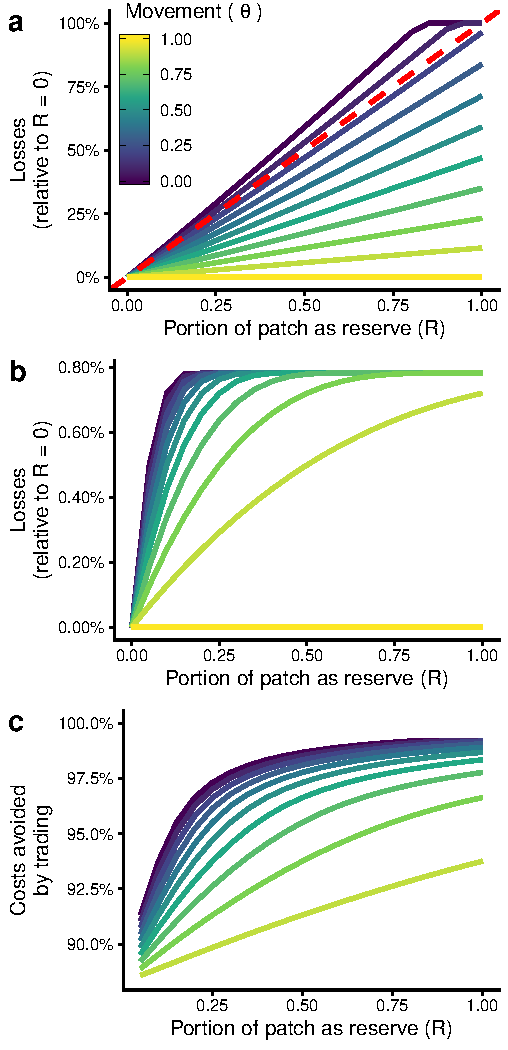
\includegraphics{img/PNA_model.pdf}
\caption{\label{fig:PNA_model}Cost of spatial closures in a vessel-day fishery (vertical axis) as a function of reserve size ($R$; horizontal axis) and movement ($\theta$; line color). Costs are shown for Patch 1 when there is no trading (A) and when trading is allowed (B). Costs avoided by trading are shown in (C). Dashed red line is a 45 degree line.}
\end{figure}

% Costs of different allocation rules
\begin{figure}[htbp]
\centering
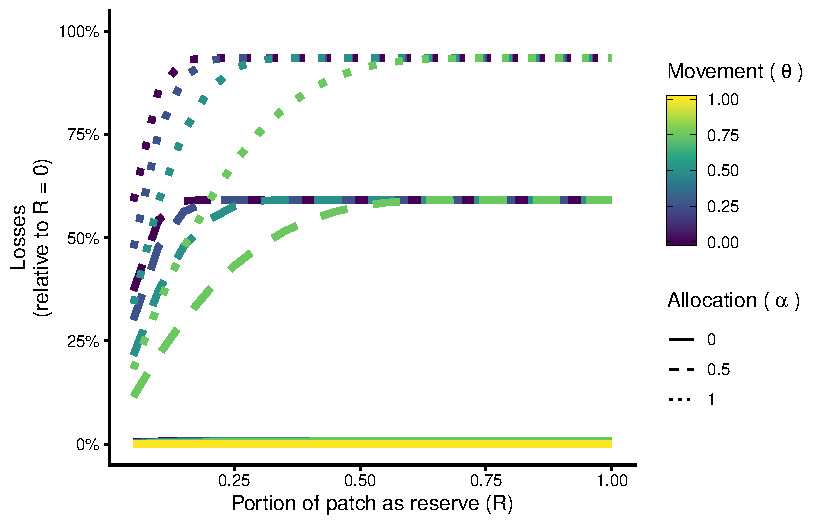
\includegraphics{img/allocation_cost_plot.pdf}
\caption{\label{fig:allocation_cost_plot}Cost (vertical axis) of different allocation rules (line colors) as a function of reserve  size ($R$; horizontal axis) and movement ($\theta$; line type). Costs are shown for Patch 1 only.}
\end{figure}

% Map of LSMPAS in PNA
\begin{figure}
\centering
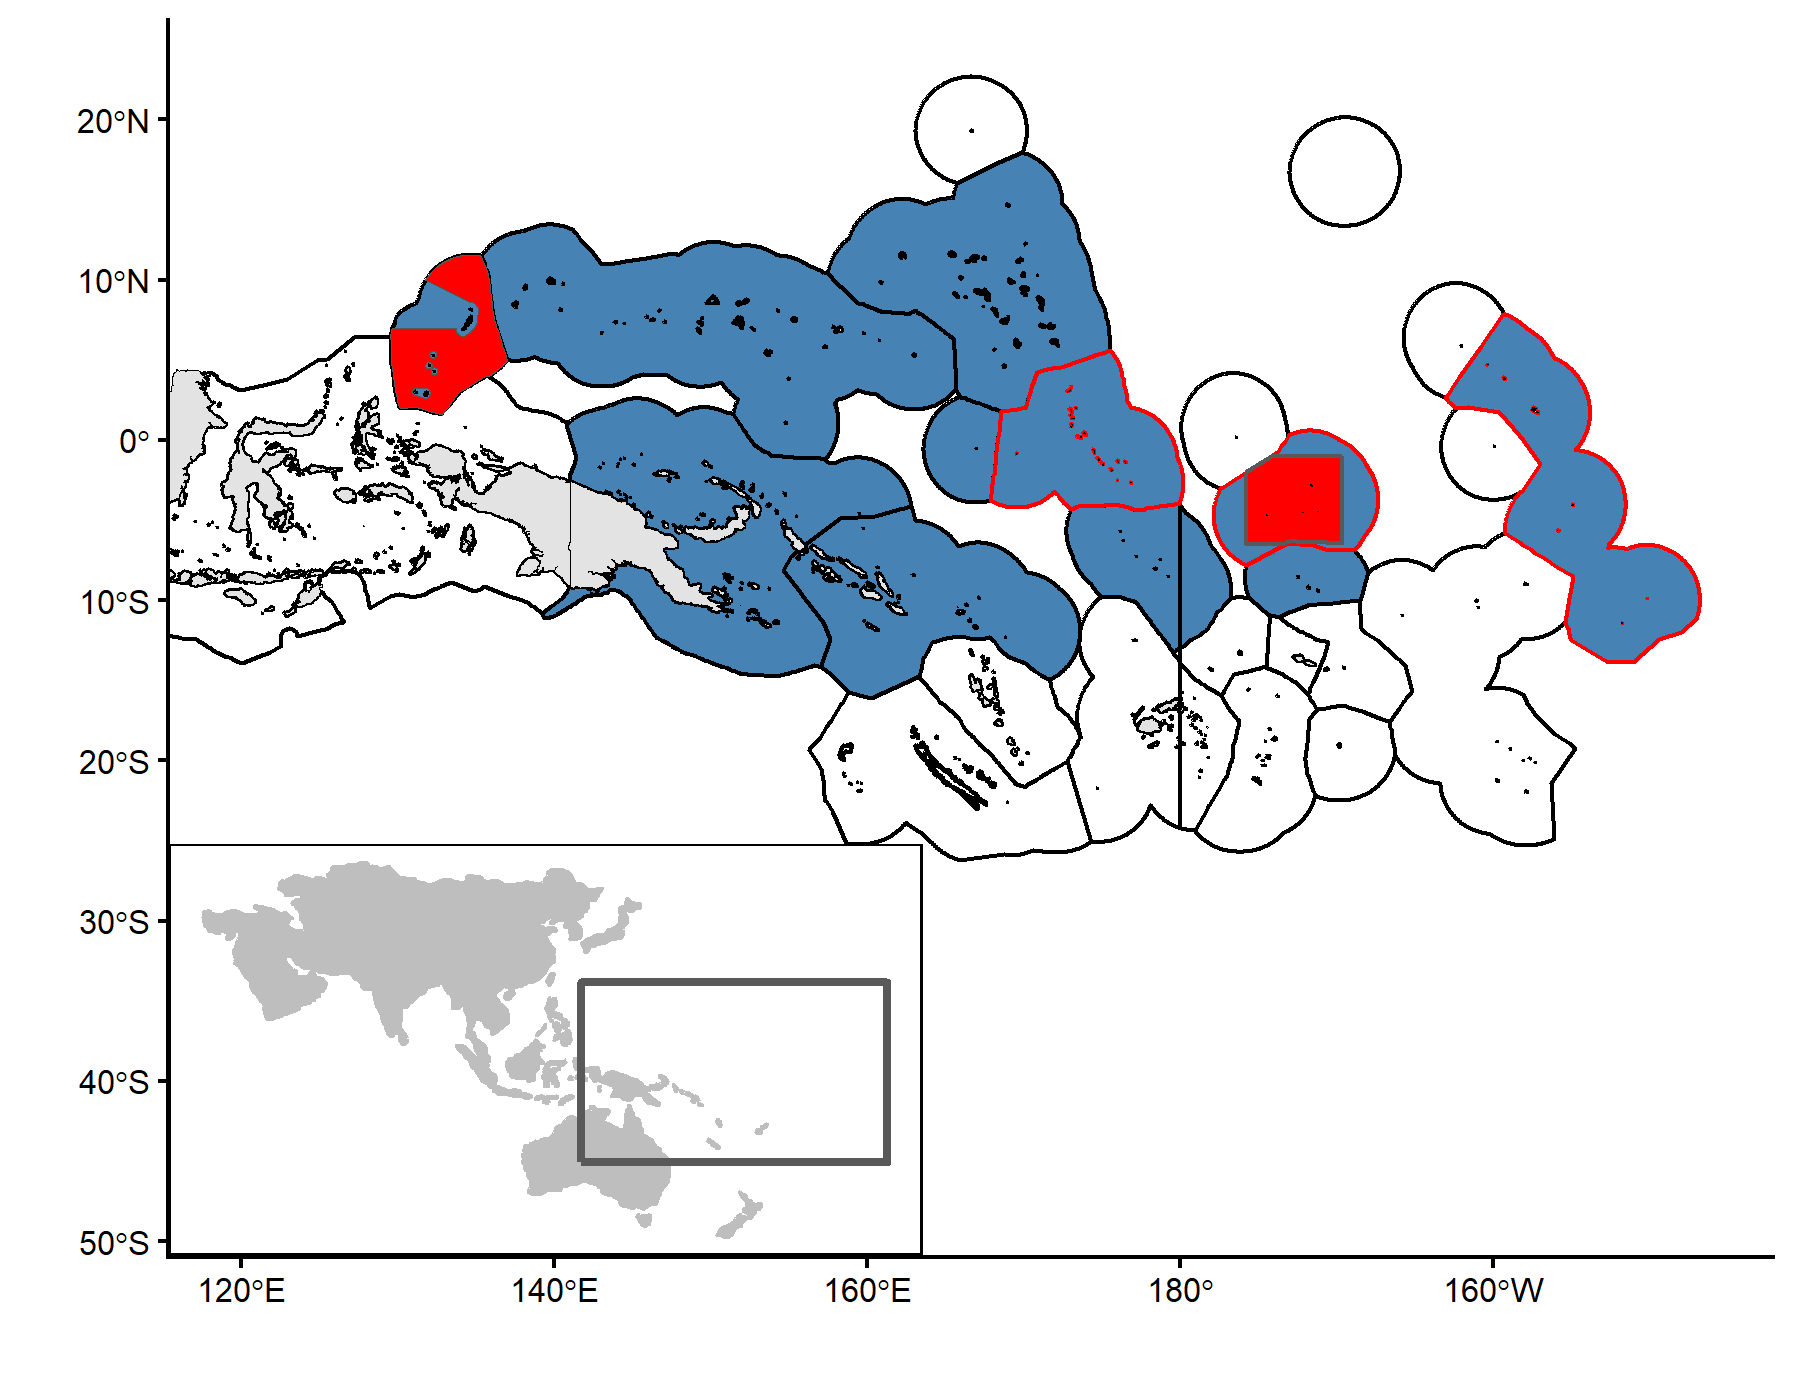
\includegraphics{img/PNA_map.png}
\caption{\label{fig:PNA_map}Map of the Exclusive Economic Zones (EEZs) of the region of interest. Countries that belong to the PNA are shown in blue, while empty polygons indicate all others. A red line indicates the Kiribati EEZ, and a solid red polygon shows PIPA. A solid purple polygon shows PNMS. Land masses are shown in gray. Labels indicate ISO3 country codes (PLW: Palau, PNG: Papua New Guinea, FSM: Federal States of Micronesia, SLB: Solomon Islands, NRU: Nauru, MHL: Marshal Islands, KIR: Kiribati, TUV: Tuvalu, TKL: Tokelau).}
\end{figure}

% Effort redistribution bars for PNA and KIR
\begin{figure}[htbp]
\centering
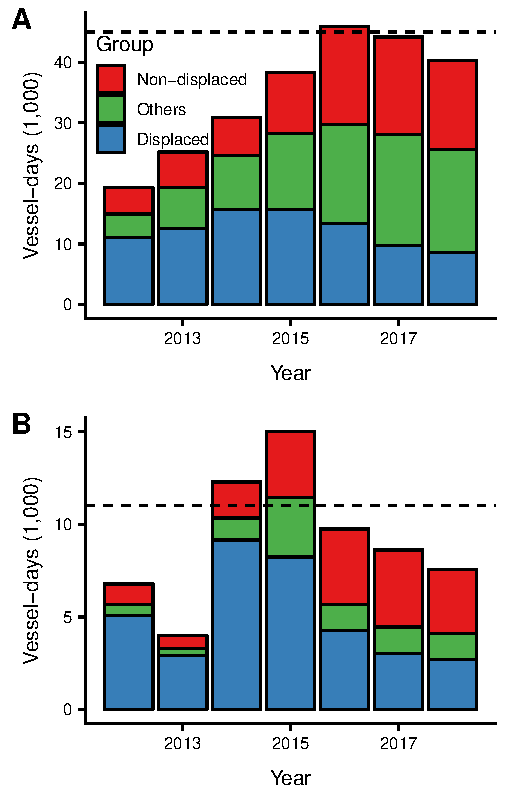
\includegraphics{img/all_PS_VDS_PNA_KIR_year.pdf}
\caption{\label{fig:all_PS_VDS_year}Observed vessel-days for Kiribati (A) and all PNA countries (B) for displaced, non-displaced, and other vessels. The dashed horizontal lines represent the total allowable effort in Kiribati (11,000 days) and the PNA (45,000 days). Note that the reduction for Kiribati is driven by displaced vessels fishing less in Kiribati's waters, but that their decrease is not as sharp for all PNA waters. Vessels displaced from PIPA fish less within the PNA, but non-displaced and other vessels fish more, resulting in a net increase.}
\end{figure}

% Revenue data from FFA and GFW estimates.
\begin{figure}[htbp]
\centering
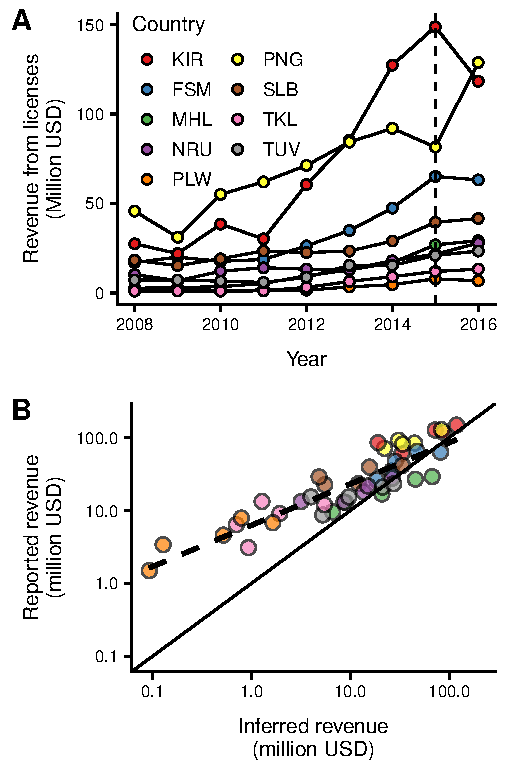
\includegraphics{img/revenues.pdf}
\caption{\label{fig:revenues}
License revenue for PNA countries. A) Annual revenue from fishing license fees by country and year (2008 - 2016) B) $log_{10}$-transformed FFA-reported revenues vs. the revenues inferred from vessel activity observations (2012 - 2016). The dashed line represents line of best fit, solid line represents 1:1 line. The same graph using absolute values is shown in \ref{fig:revenue_FFA_GFW_linear}. A graph showing reported revenues and observed effort is shown in \ref{fig:revenue_FFA_effort_GFW}.}
\end{figure}

% Palau Raster and PNMS
\begin{figure}
\centering
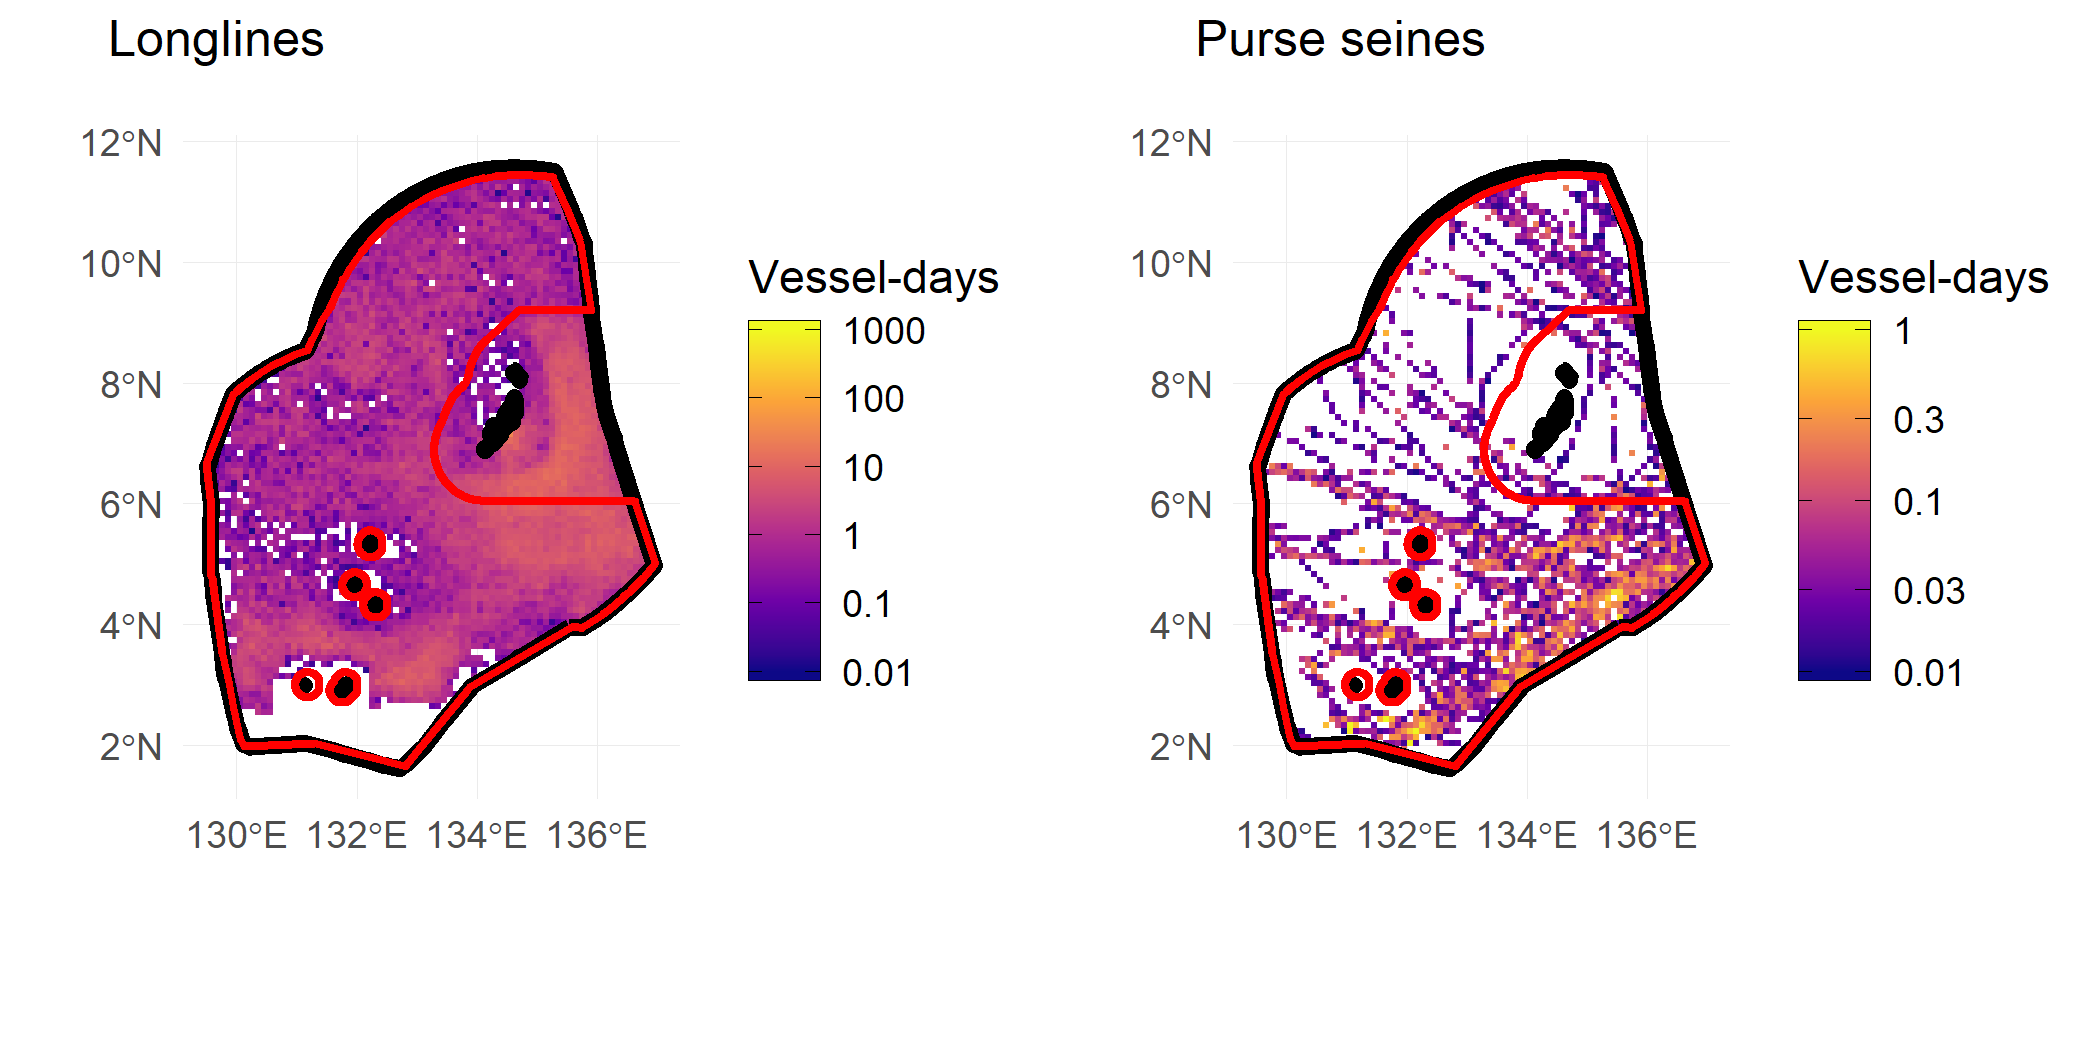
\includegraphics{img/plw_2018.png}
\caption{\label{fig:plw_2018}Longline and purse seine fishing effort in Palau during 2018 at a 0.5 degree resolution. The red polygon shows the Palau National Marine Sanctuary, containing 56\% and 91\% of longline and purse seine fishing effort, respectively.}
\end{figure}

%%%%%%%%%%%%%%%%%%%%%%%%%%%%%%%%%%%%%%%%%
%%%%%%%%%%%%%		 					 %%%%%%%%%%%%%
%%%%%%%%%%%%%		 BEGIN APPENDIX		 %%%%%%%%%%%%%
%%%%%%%%%%%%%		 					 %%%%%%%%%%%%%
%%%%%%%%%%%%%%%%%%%%%%%%%%%%%%%%%%%%%%%%%

\clearpage

\FloatBarrier

\newcommand{\beginsupplement}{\setcounter{table}{0}  \renewcommand{\thetable}{S\arabic{table}} \setcounter{figure}{0} \renewcommand{\thefigure}{S\arabic{figure}}}

\setcounter{table}{0}  \renewcommand{\thetable}{S\arabic{table}} \setcounter{figure}{0} \renewcommand{\thefigure}{S\arabic{figure}}

\section{Supplementary Materials}

\subsection{Model for marine conservation with effort markets}

We model a ten-patch discrete-time meta-population system, where Patch 1 is considering a spatial closure. Patches 1 - 9 opperate under a vessel-day schemePatches, and Patch 10 represents the high seas and other areas not managed under a VDS. The stock of fish in each country is relatively stationary within a single fishing season, but redistributes across all patches annually. The price of fish is $p$, and catchability is given by $q$. These parameters are held constant across patches.

\subsubsection{Fishery dynamics}

In the absence of a reserve, the revenue for vessels in patch $i$ is given by $pqE_iX_i$, where $E_i$ and $X_i$ are effort (vessel-days) and stock size in patch $i$ at the beginning of a period. The cost of fishing in patch $i$ is given by $cE_i^\beta$, where $\beta = 1.3$ matches commonly-used cost functions.

Patch 1 considers a spatial closure by implementing a reserve as a fraction $R$ of the total patch ($R \in[0,1)$). Fish move within a patch based on $\theta$, where $\theta = 0$ implies no movement within the patch, and $\theta = 1$ implies that fish within the patch are well mixed during the fishing season. In this patch, revenues are given by $pqE_1X1(\theta + (1 - \theta)(1 - R))$. The parameterization of movement and reserve size imply that profit from fishing Patch 1 is given by:

$$
\Pi_1(E_1,X_1,R) = pqE_1X_1\Omega_1-cE_1^\beta
$$

With $\Omega_1 = (\theta + (1 - \theta)(1 - R))$ being a parameterization that combines reserve size as a proportion of patch ($R =  (0, 1)$) and within-patch fish movement ($\theta$). Under this parameterization, $\Omega_{i \neq 1} = 1$ since only Patch 1 implements a reserve.

Therefore, profits from fishing in patches 2 - 10 are:

$$
\Pi_i(E_i,X_i) = pqE_iX_i\Omega_i-cE_i^\beta
$$

The above equations imply that the marginal profit from the last unit of effort in a patch are given by:

$$
\pi_1(E_1) = pqX_1\Omega_i - \beta cE_1^{\beta-1}
\label{eqn:marginal_profit}
$$

In practice, the effort levels in each Patch are allocated by management (so $E_{1},\ E_{2},...,E_{9}$ are given) and the
effort level on the high seas ($E_{10}$) is a result of open access dynamics. Therefore, we assume that effort continues to enter Patch 10 until the profit from the last unit of effort is exactly zero, indicating that $E_{10}$ is the value for which $\pi_{10}(E_{10})  = 0$. Setting Equation \ref{eqn:marginal_profit} for $i = 10$ equal to zero and removing $\Omega_{10} = 1$ for simplicity, we can solve for $E_{10}$:

$$
E_{10} = \left(\frac{pqX_{10}}{\beta c}\right)^{\frac{1}{(\beta - 1)}}
\label{eqn:effort_hs}
$$

Under vds-operated patches, however, profits from marginal effort must equate the cost of fishing in the patch. Therefore vessel-day price for patches under vds ($i = (1, 9)$) is  given by:

$$
\pi(E_i) = pqX_i\Omega_i - \beta c E_i ^{\beta - 1}
$$

We can solve for $E_i$ and obtain:

\begin{equation}
	\begin{split}
		\pi_i + \beta c E_i ^{\beta - 1} &= pqX_i\Omega_i \\
		\beta c E_i ^{\beta - 1} &= pqX_i\Omega_i - \pi_i \\
		E_i ^{\beta - 1} &= \frac{pqX_i\Omega_i - \pi_1}{\beta c} \\
		E_i &= \left(\frac{pqX_i\Omega_i - \pi_1}{\beta c }\right) ^ {\frac{1}{\beta - 1}}
	\end{split}
\label{eqn:demands}
\end{equation}

Therefore, total allowable effort in the fishery is given by:

$$
\bar{E} = \sum_{i = 1}^9\left(\frac{pqX_i\Omega_i - \pi}{\beta c }\right) ^ {\frac{1}{\beta - 1}}
\label{eqn:Ebar}
$$

\subsubsection{Stock dynamics}

Patch-level harvest is then determined by effort and stock size:

$$
H_i = qE_iX_i\Omega_i
\label{eqn:harvest}
$$

Therefore, escapement in patch $i$ is the difference between initial stock size and harvests given by $e_{it} = X{it} - H_{it}$ and total escapement is $e_t=\sum_{i=1}^{10}e_{it}$. The entire stock then grows logistically according to:

$$
X_{t+1} = e_t + e^{r \times \frac{e}{K}}
\label{eqn:grow}
$$

Where $r$ and $K$ are species-specific intrinsic growth rate and carrying capacity.

After the stock grows, a constant and patch-specific fraction $f_i$ of the total stock redistributes to patch $i$, so:

$$
X_{it+1} = f_iX_{t+1}
\label{eqn:disperse}
$$

\subsubsection{Vessel-day revenues}

The vessel-day price that a country charges is given by $\pi_i$ from Eqn \ref{eqn:marginal_profit}. Therefore, patch-level license revenues are given by:

$$
\omega = \pi_iE_i
\label{eqn:license_revenue}
$$

Equation \ref{eqn:harvest} shows that low values of $\theta$ and $R > 0$ would increase escapement, which would lead to an increase in stock size (Equation \ref{eqn:grow}) and a benefit to all the other patches. But this would also cause the stock in the high seas ($X_{10}$) to increase, leading to an increased effort being allocated to the high seas (Equation \ref{eqn:effort_hs}) and a loss of these potential rents. Thus, the spillover benefits of increasing $R$ are never completely captured.

\subsubsection{Simulations and parametrization}

We inform our model to losely match the fishery dynamics observed for the VDS operated by the PNA. The table below contains the values used to parameterize the model.


\begin{tabular}{l|r|l}
\hline
Parameter & Value & Source\\
\hline
MSY & 1.875600e+06 & 50th percentile from MSY in table 8 of Stock Assessment\\
\hline
$B_{msy}$ & 1.628000e+06 & 50th percentile from MSY in table 8 of Stock Assessment\\
\hline
K & 6.876526e+06 & 50th percentile from MSY in table 8 of Stock Assessment\\
\hline
$B_c/B_{msy}$ & 5.100000e-01 & 50th percentile from MSY in table 8 of Stock Assessment\\
\hline
$C_{now}$ & 1.679444e+06 & Catches from Stock Assessment\\
\hline
$B_{now}$ & 3.507028e+06 & Current Biomass (2012 - 2015 average)\\
\hline
$r$ & 5.700000e-01 & From fishbase: Prior r = 0.57, 95 CL = 0.41 - 0.78\\
\hline
$\beta$ & 1.300000e+00 & Standard\\
\hline
p & 1.100000e+03 & Mean between Thailand and Japan values (Value of WCPFC-CA tuna fisheries 2017 report)\\
\hline
q & 3.420000e-05 & Estimated so that efforts match catches given biomass and vessel-day prices\\
\hline
c & 1.800000e+02 & -\\
\hline
f & 1.000000e-01 & Biomass is equally distributed between patches ($f_i = 0.1$)\\
\hline
\end{tabular}

We use the model above run three different simulations. We test the model across a range reserve sizes and movement parameters. We use to main scenarios. The first scenario does not allow trading. In this case, total allowable effort ($\bar{E}$) and biomass $B_{now}$ are known and equally distributed among patches 1-9. For patch 10, we solve for Eq \ref{eqn:effort_hs} until biomass converges to match $B_{now}$. We then proceed to ``close'' a portion of Patch 1, and calculate the vessel-day price in Patch 1 given that only $X_i\Omega_i$ biomass is available for harvest. We compare vessel-day revenues of each scenario to a case with no reserve ($R = 0$). This produces a measure of the cost of implementing a spatial closure of size $R$ in patch 1.

The second scenario allows trading. We start again by solving for the high seas to obtain total effort. Since a closure is not in effect, this equiulibrium is the same as the first step above. We then implement a spatial closure in patch 1. This essentially lowers the price fishers would be willing to pay to fish in a patch with biomass $X_i\Omega_i$, lowering demand for vessel-days in pach 1. Patches 2 - 9 have a higher demand for vessel days, and therefore a portion of vessel-days from patch 1 are sold to patches 2 - 9. This increases effort in these patches, which reduces escapement and therefore biomass. This reduction in biomass in turn would modify the demand curves (Eq \ref{eqn:demands}). We therefore iterate this process until biomass stabilizes, therefore finding the system's equilibrium. Like before, we calculate vessel-day revenues to each patch and compare them to a case with no reserve in patch 1.

\subsection{Allocation rules}

Annual vessel-days are often allocated based on a combination of historical within-patch effort and biomass. In the PNA, for example, sixty percent of the allocation is calculated based on EEZ effort over the last seven years and 40\% is calculated based on the 10-year average of each country’s share of estimated skipjack and yellowfin biomass within its EEZ.\footnote{This is explained in more detail in Article 12.5 of the 2012 Amendment to the Palau Agreement and in \cite{Hagrannsoknir2014}.} Trading vessel-days to other countries would imply that historical within-patch effort declines through time. The allocated days to a patch with a full spatial closure would eventually be reduced to just the 40\% based on biomass.

In the second scenario above, effort from a patch with conservation is traded to other patches. This means that its allocation will decrease as purse seine effort in its EEZ is reduced. After solving for the new equilibrium for each combination of $R$ and $\theta$, we project the fishery 50 years in time. At the end of every time, vessel-days are allocated to each patch based on the following rule:

$$
E_i^* = \alpha \left(\frac{\sum_{\tau = 0}^{\hat{\tau}}E_{i,t-\tau}}{\bar{E}\hat{\tau}} \right) +
(1 - \alpha) \left(\frac{\sum_{\tau = 0}^{\hat{\tau}}X_{i,t-\tau}}{\bar{X}\hat{\tau}} \right)
$$

Where  $\alpha$ is a weight on historical effort ($E_i$) and $1-\alpha$ is the weight in historical biomass ($B_i$). We use $\hat{\tau}= 7$ to obtain a moving mean of 7 years for these measures. The difference between allocated days ($E_i^*$) and used days (determined by Eq: \ref{eqn:demands}) for patch 1 are the sales. We then calculate vessel-day revenues to each country over the 50-year time horizon and compare them to a case where there is no reserve and allocations are based solely on biomass ($\alpha = 0$).

\subsection{Data}

Automatic Identification Systems (AIS) are on-board devices that provide at-sea safety and prevent ship collisions by broadcasting vessel position, course, and activity to surrounding vessels. These broadcast messages can be received by satellites and land-based antennas. GFW then uses machine learning algorithms (convolutional neural networks) on the broadcast messages to infer type and location of fishing events \cite{kroodsma_2018}

The amount of data gathered by GFW is dependent on the number of antennas and satellites that can receive signals. The total satellite count increased from 3 to 6 on June 1\textsuperscript{st} 2014 , and then from 6 to 10 on January 1\textsuperscript{st} 2016. This causes an increase in the number of \emph{received} AIS messages (\emph{i.e.} points), and therefore an apparent increase in the number of vessels and vessel activity. The addition of new satellites affects all vessels in the same way.

Our displaced group contains all purse seiners (n = 64) that fished within PIPA at least once before the announcement, and that continued to fish elsewhere after the January 2015 implementation. Vessels in the non-displaced group meet the following two conditions: i) never fished within PIPA waters from 2012-2015, and ii) vessels have fished in surrounding areas (\emph{i.e.} PNA-countries' EEZ) before and after PIPA closure (n = 28). Together, these vessels represent more than 20 million geo-referenced positions for which we know activity (fishing or not fishing). We perform three sample restrictions as a robustness check. The first restriction excludes all Chinese vessels, the second excludes all PNA vessels, and the third excludes US and Taiwanese vessels.

\subsection{Analysis}

ENSO events are known to drive the location of fish and behavior of fishing vessels, especially in PNA waters \cite{lehodey_1997,kroodsma_2018,aqorau_2018}. We do our best to control for these environmental changes by incorporating the NINO4 anomaly index in our analyses, and by tracking the non-displaced vessels as a ``control'' group that is equally affected by the environmental variation. For example, we observe that both displaced and non-displaced vessels shifted their effort post-PIPA to the Western margin of the PNA region, namely Kiribati's Gilbert Islands and Tuvalu. However, displaced vessels redistribute a greater proportion of fishing effort to these areas, as well as the High Seas (Fig \ref{fig:fishing_raster_diff}). Our analysis shows that sea surface temperature variation does have an effect on our crowding and behavioral outcomes, but that by itself it does not explain the observed patterns. While environmental variation certainly influences fishing behavior, policy and management interventions such as moratoriums and spatial closures can have even larger effects \cite{kroodsma_2018}.  Our analyses incorporate the monthly NINO4 anomaly index (Fig. \ref{fig:nino_plot}) to control for the association that fish and vessels might have to environmental variation \cite{lehodey_1997,kroodsma_2018,aqorau_2018}.

\subsubsection{Crowding effect}

$$
y_t = \alpha + \beta_1 M_t + \beta_2 M_t^2 + \beta_3 M_t^3 + \beta_4 M_t ^4 + \sigma_s + \mu N_t + \epsilon_t
\label{eqn:sp_corr}
$$

We test for a crowding effect using the specification in Equation \ref{eqn:sp_corr}. We have two different outcome variables:
1) the number of cells that had fishing activity from displaced and non-displaced vessels per month and 2) the correlation of presence/absence of fishing events between both groups over one month.We allow for the possibility of three inflection points: 1) initial crowding due to MPA implementation, 2) When the crowding has reached its peak and starts to decrease, and 3) when this decrease potentially levels off. For this reason, we fit a 4th degree polynomial to our monthly indices. We do so by centering our time series of crowding indices on the day of implementation. Our explanatory variable is therefore the number of months ($M$) before or after the implementation. For example, since PIPA was implemented in January 1st of 2015, December of 2014 has a value of -1 and Feb of 2015 would receive a value of 1. Note that we restrict the sample to our displaced and non-displaced vessels (vessels that show up in the dataset before PIPA implementation) to try to minimize bias from more and more vessels using AIS over time. We also include controls ($\sigma_s$) that captures the effect of additional satellites receiving AIS signals, which occurred on April 1st, 2014 and December 31st, 2015. The $\mu$ coefficient captures the effect of the NINO4 anomaly.

\subsubsection{Behavioral changes}

We attempt to identify the response of vessels to the PIPA closure. We use daily fishing and non-fishing hours, daily proportion of fishing vs. non-fishing hours, daily distance traveled (km), distance from shore (km) and distance from home port (km) for fishing events, and proportion of total fishing hours allocated to Kiribati waters and PNA waters as our main outcomes of interest. We compare these outcomes before and after the implementation of PIPA using a Difference-in-Differences approach.

Our main specification is the following:

$$
log(y_{i,t}) = \alpha + \beta_1 P_t + \beta_2 D_i + \beta_3 P_t \times D_i + \phi_t + \gamma_i + \epsilon_{i,t}
\label{eqn:did}
$$

\noindent where $log(y_{i,t})$ is the hyperbolic-sine transformation\footnote{$ln\left(y + \sqrt{1 + y^2}\right)\rightarrow ln(2y)$ the transformation was not applied to the proportion of fishing to non-fishing hours.} of the outcome of interest for vessel $i$ on period $t$. A dummy variable $P_t$ takes the value of 0 for all dates prior to PIPA implementation and a value of 1 for all dates following PIPA implementation. $D_i$ is a dummy variable indicating whether a vessel belongs to the displaced ($D_i = 1$) or non-displaced ($D_i = 0$) group. $\alpha$ is the standard intercept term, $\beta_1$ captures the temporal trend, $\beta_2$ captures the initial difference between displaced and non-displaced groups, and $\beta_3$ is our parameter of interest: the difference-in-differences estimate capturing the treatment effect. Finally, $\phi_t$ and $\gamma_i$ represent month and flag dummies that account for seasonality or country-level management interventions.

All regression coefficients were estimated via ordinary least squares, and heteroskedasticity-robust standard errors were calculated. All analyses were performed in R version 3.5.1 \cite{rcore_2018}. Raw data and code used in this work are available on \href{https://github.com/jcvdav/MPA_displacement}{github}.

\subsubsection{Revenues and catches}

We obtained information on revenues from the Pacific Islands Forum Fisheries Agency \emph{Tuna Development Indicators 2016} report.  Specifically, we use data compiled by the Pacific Islands Forum Fisheries Agency (FFA\footnote{https://www.ffa.int/node/2050}) where annual revenues from license fees (for VDS and other access programs) are reported for each country (2008 - 2016; Fig. \ref{fig:revenues}A). For countries in the PNA, these revenues show a combination of vessel-day license fees as well as joint-venture operations.

Total purse seine catch for each country's EEZ for the 1997 - 2016 period were also obtained from the FFA (Fig. \ref{fig:catches}). Catches in Kiribati waters decreased from 24,051 to 12,894 tonnes between 2015 and 2016 (46.3\% decrease). Similar decreases were observed for The Federated States of Micronesia (60.9\%), Papua New Guinea (43.4\%) and the Solomon Islands (58.5\%). In contrast, Tokelau (due south of PIPA) showed a 22.3\% increase in purse seine catch over the same period.

\clearpage

\section{Supplementary tables and figures}

\begin{figure}
\centering
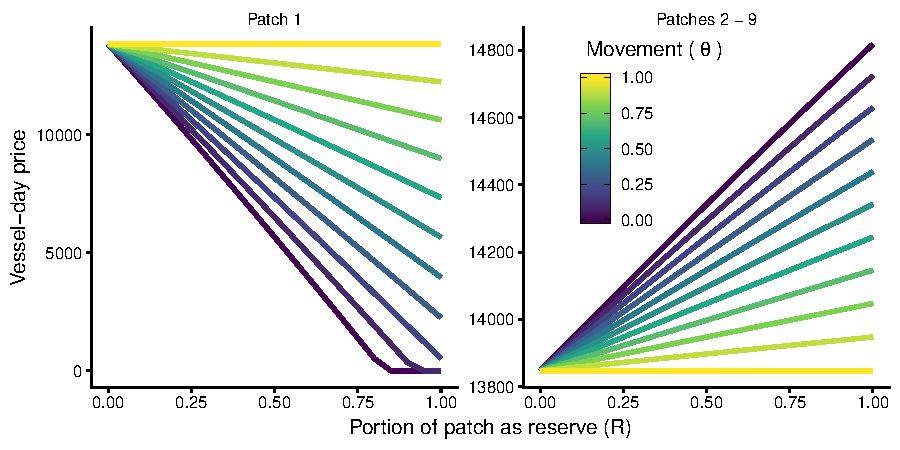
\includegraphics{img/vessel_day_price_no_trading_plot.pdf}
\caption{\label{fig:vessel_day_price_no_trading_plot}Vessel-day prices (vertical axis) for a combination of reserve sizes ($R$ in the horizontal-axis) and different within-patch movement ($theta$) for the patch with spatial closure and other patches (left - right, respectively) when there is no trading.}
\end{figure}

\begin{figure}
\centering
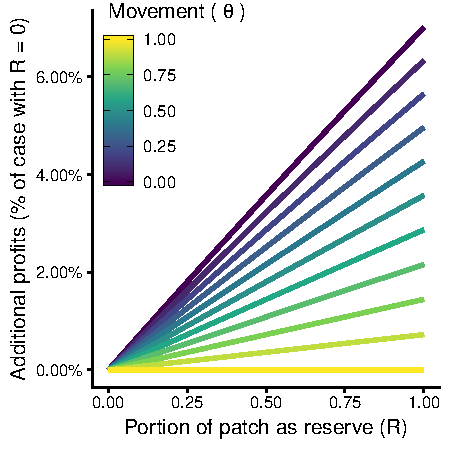
\includegraphics{img/profits_PNA_notKIR_no_trading_plot.pdf}
\caption{\label{fig:profits_PNA_notKIR_no_trading_plot}Relative change in revenue for patches 2 - 9 (vertical axis) for a combination of reserve sizes ($R$ in the horizontal-axis) and different within-patch movement ($theta$) when there is no trading.}
\end{figure}

\begin{figure}
\centering
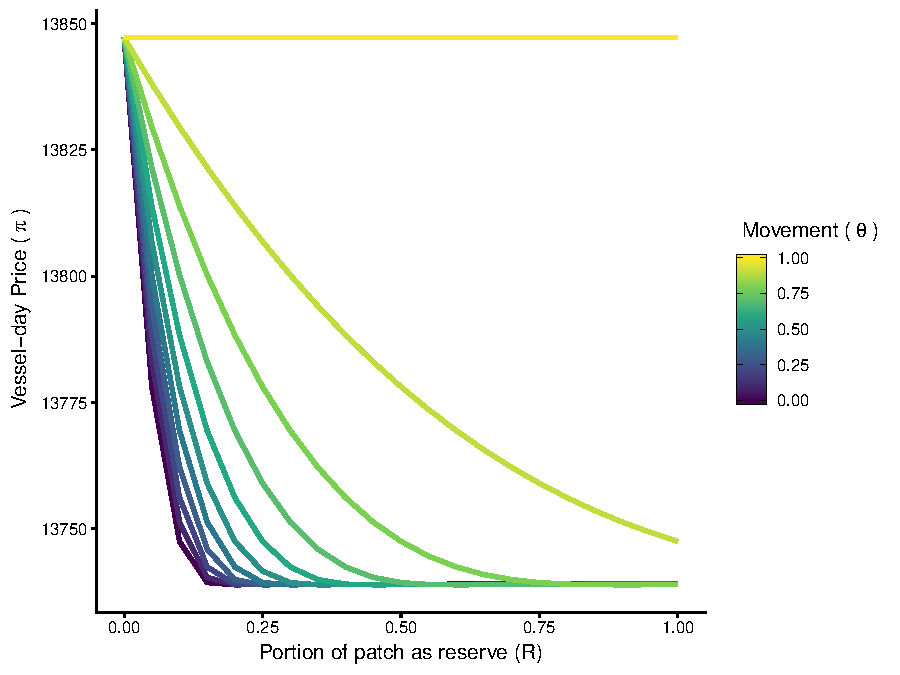
\includegraphics{img/vessel_day_price_with_trading_plot.pdf}
\caption{\label{fig:vessel_day_price_with_trading_plot}Vessel-day prices (vertical axis) for a combination of reserve sizes ($R$ in the horizontal-axis) and different within-patch movement ($theta$) for the patch with spatial closure and other patches (left - right, respectively) when there is no trading.}
\end{figure}

\begin{figure}
\centering
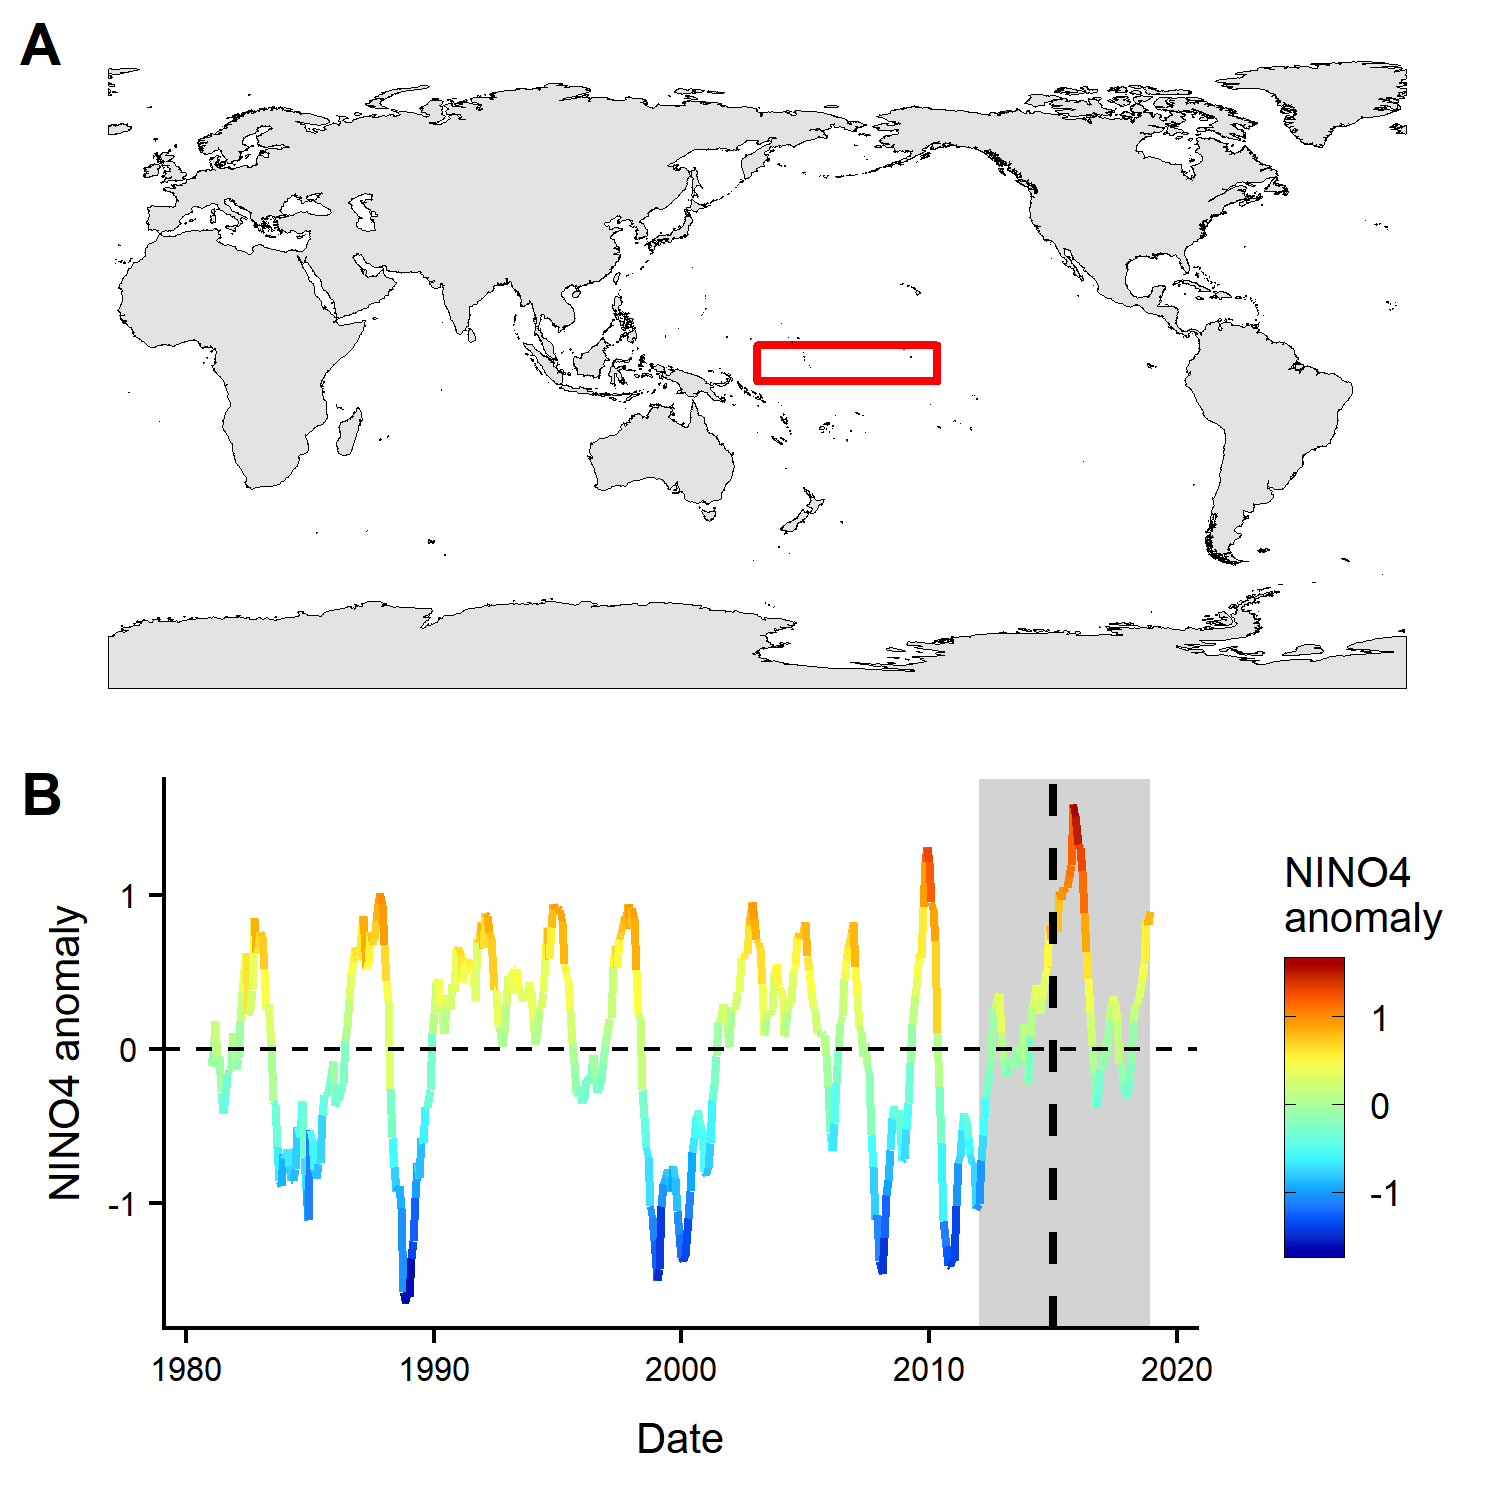
\includegraphics{img/nino_plot.png}
\caption{\label{fig:nino_plot}NINO4 anomaly index. A) Map of the NINO4 region (5S-5N and 160E-150W). B) Timeseries of NINO4 anomaly from January, 1980 to December, 2018.}
\end{figure}

\clearpage

We can compare the footprint of displaced and non-displaced vessels before and after the implementation of PIPA to understand effort redistribution. Non-displaced vessels serve serve as a control group that was not subject to a spatial closure but might have redistributed in response to changing environmental conditions, such as ENSO. The spatial redistribution patterns of displaced vessels relative to non-displaced vessels suggest that some relocated to other waters in Kiribati (\emph{i.e.} Gilbert islands and Line islands), but also the Marshal Islands and the high seas (Fig \ref{fig:fishing_raster_diff}).

\begin{figure}
\centering
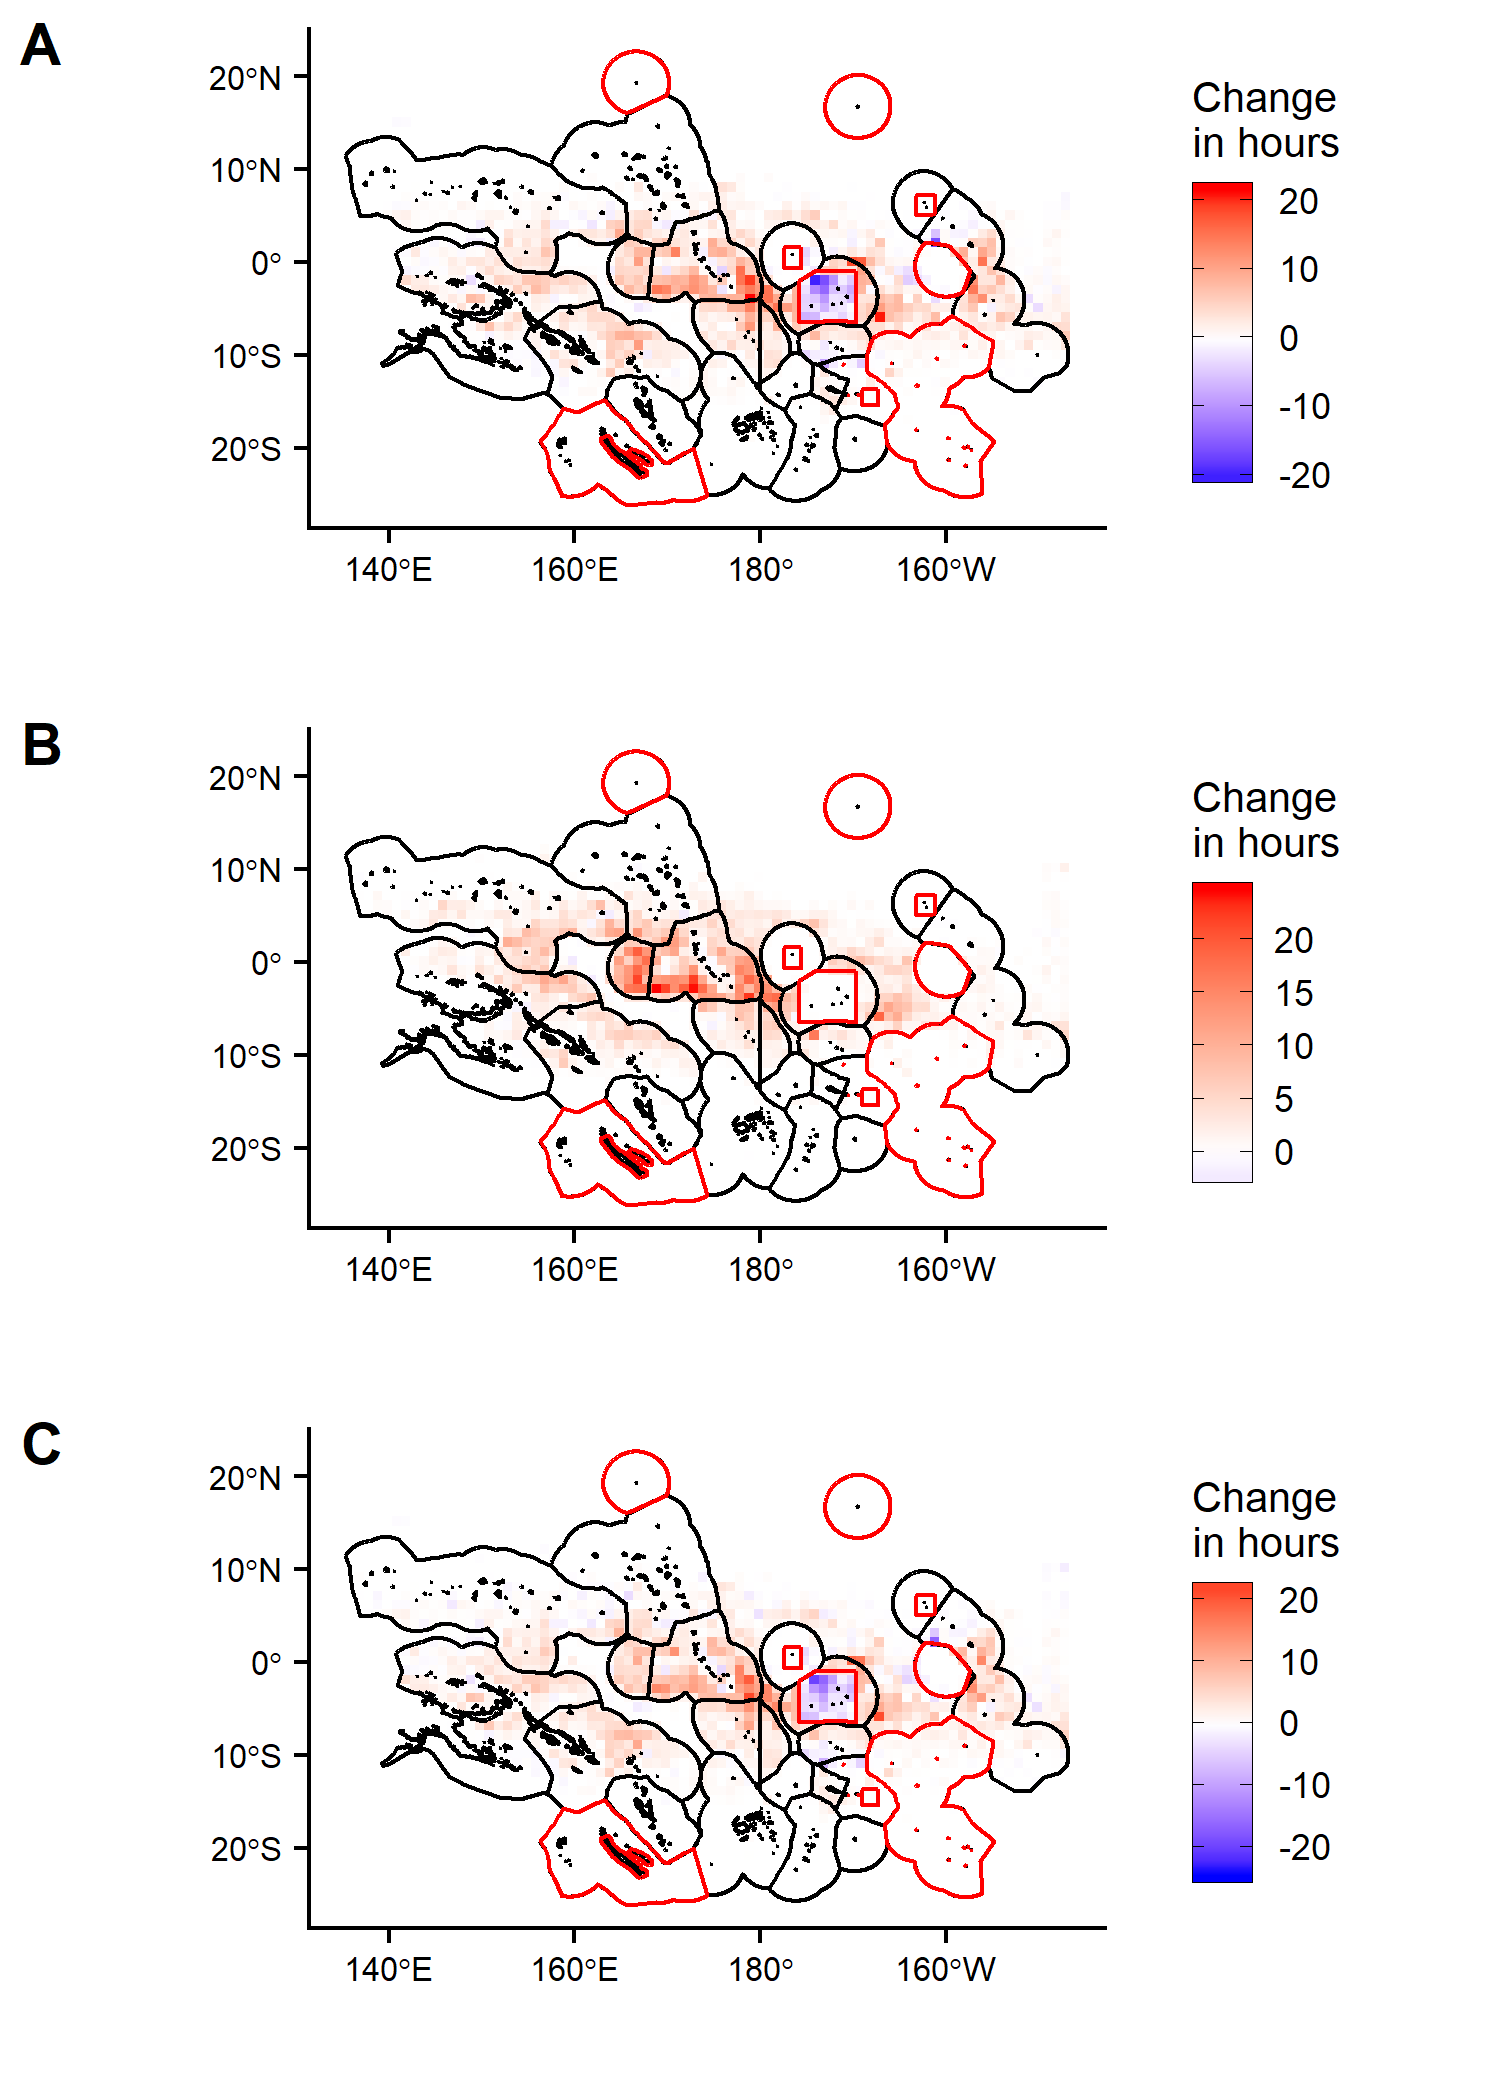
\includegraphics{img/fishing_raster_diff.png}
\caption{\label{fig:fishing_raster_diff}Change in spatial footprint of analyzed vessels. Black lines show Exclusive Economic Zone (EEZ), red lines show existing Marine Protected Areas. Panels A and B show the change through time (after - before) for displaced (A) and non-displaced vessels (B). Panel C shows the difference between A and B (displaced - non-displaced), highlighting areas where displaced vessels redistributed to, relative to non-displaced vessels. Note that displaced vessels allocate more hours to the Gilbert Islands and Line islands EEZs, but also Tuvalu and the high seas surrounding PIPA and Kiribati's EEZ.}
\end{figure}

\begin{landscape}

\begin{table}[!htbp] \centering 
  \caption{\label{tab:sp_corr}Coefficient estimates for a third-polinomial fit to the measures of crowding. The first column shows coefficients for the number of cells with treated and control vessels during the same month. The second column shows coefficients for the spatial correlation for presence / absence of treated and control vessels. The explanatory variable is the number of months before implementation of PIPA. Numbers in parentheses are heteroskedastic-robust standard errors.} 
  \label{} 
\footnotesize 
\begin{tabular}{@{\extracolsep{1pt}}lcccccccc} 
\\[-1.8ex]\hline 
\hline \\[-1.8ex] 
\\[-1.8ex] & (1) & (2) & (3) & (4) & (5) & (6) & (7) & (8)\\ 
\hline \\[-1.8ex] 
 Constant & 78.040$^{***}$ & 84.639$^{***}$ & 60.962$^{***}$ & 66.725$^{***}$ & 0.412$^{***}$ & 0.417$^{***}$ & 0.370$^{***}$ & 0.377$^{***}$ \\ 
  & (5.438) & (8.990) & (15.598) & (15.988) & (0.014) & (0.032) & (0.062) & (0.066) \\ 
  & & & & & & & & \\ 
 M & 3.943$^{***}$ & 4.065$^{***}$ & 3.066$^{***}$ & 3.139$^{***}$ & 0.010$^{***}$ & 0.010$^{***}$ & 0.009$^{**}$ & 0.009$^{**}$ \\ 
  & (0.302) & (0.348) & (0.966) & (1.040) & (0.001) & (0.001) & (0.003) & (0.004) \\ 
  & & & & & & & & \\ 
 M $^2$ & $-$0.005 & $-$0.021 & 0.008 & $-$0.008 & $-$0.0001$^{***}$ & $-$0.0001 & $-$0.0001 & $-$0.0001 \\ 
  & (0.019) & (0.026) & (0.027) & (0.030) & (0.00004) & (0.0001) & (0.0001) & (0.0001) \\ 
  & & & & & & & & \\ 
 M $^3$ & $-$0.002$^{***}$ & $-$0.002$^{***}$ & $-$0.002$^{***}$ & $-$0.002$^{***}$ & $-$0.00001$^{***}$ & $-$0.00001$^{***}$ & $-$0.00001$^{***}$ & $-$0.00001$^{***}$ \\ 
  & (0.0003) & (0.0003) & (0.001) & (0.001) & (0.00000) & (0.00000) & (0.00000) & (0.00000) \\ 
  & & & & & & & & \\ 
 M $^4$ & 0.00001 & 0.00002 & 0.00000 & 0.00001 & 0.00000$^{***}$ & 0.00000$^{**}$ & 0.00000 & 0.00000 \\ 
  & (0.00001) & (0.00002) & (0.00002) & (0.00002) & (0.00000) & (0.00000) & (0.00000) & (0.00000) \\ 
  & & & & & & & & \\ 
 NINO4 &  & $-$8.095 &  & $-$10.395 &  & $-$0.006 &  & $-$0.014 \\ 
  &  & (8.287) &  & (9.481) &  & (0.029) &  & (0.031) \\ 
  & & & & & & & & \\ 
 $\sigma_1$ &  &  & 21.318 & 25.102 &  &  & 0.057 & 0.062 \\ 
  &  &  & (19.493) & (22.486) &  &  & (0.076) & (0.080) \\ 
  & & & & & & & & \\ 
 $\sigma_2$ &  &  & 5.299 & 3.194 &  &  & $-$0.015 & $-$0.018 \\ 
  &  &  & (18.874) & (18.670) &  &  & (0.035) & (0.035) \\ 
  & & & & & & & & \\ 
\hline \\[-1.8ex] 
NINO4 & No & Yes & No & Yes & No & Yes & No & Yes \\ 
Satellites & No & No & Yes & Yes &  &  &  &  \\ 
Observations & 84 & 84 & 84 & 84 & 84 & 84 & 84 & 84 \\ 
R$^{2}$ & 0.791 & 0.793 & 0.795 & 0.798 & 0.703 & 0.704 & 0.709 & 0.710 \\ 
\hline 
\hline \\[-1.8ex] 
\textit{Note:}  & \multicolumn{8}{r}{$^{*}$p$<$0.1; $^{**}$p$<$0.05; $^{***}$p$<$0.01} \\ 
\end{tabular} 
\end{table} 

\end{landscape}

\begin{figure}[htbp]
\centering
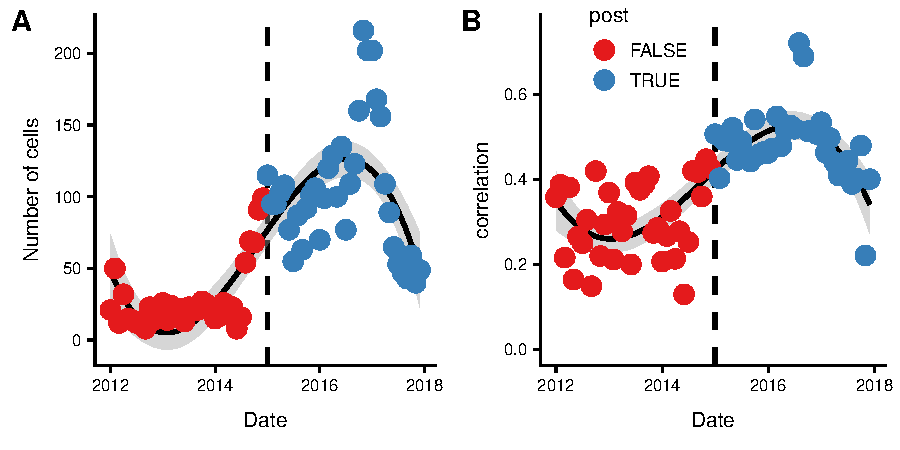
\includegraphics{img/sp_corr.pdf}
\caption{\label{fig:sp_corr}Number of cells that had displaced and non-displaced vessels (A) and spatial correlation in the presence-absence of each group per cell (B). The solid lines represent the 4\textsuperscript{th} degree polynomial fit reported in \ref{tab:sp_corr}. Note that the late 2016 and early 2017 showed negative or neutral NINO4 anomalies similar to those in the pre-PIPA period, but crowding effect does not decline to pre-implementation level and seems to stabilize.}
\end{figure}

\begin{landscape}

\begin{table}[H] \centering 
  \caption{\label{tab:KIR_sp_corr}Coefficient estimates for a fourth-degree polynomial fit to the measures of crowding for Kiribati EEZ only. The first five columns represent different specifications for number of cells with presence of both fleets. Columns 6 - 10 show coefficients for the spatial correlation for presence / absence of displaced and non-displaced vessels. The explanatory variable is the number of months before or after implementation of PIPA. Numbers in parentheses are heteroskedastic-robust standard errors. The last column of each group presents fits with only NINO4 anomaly index as an explanatory variable.} 
  \label{} 
\footnotesize 
\begin{tabular}{@{\extracolsep{0.1pt}}lcccccccccc} 
\\[-1.8ex]\hline 
\hline \\[-1.8ex] 
\\[-1.8ex] & \multicolumn{5}{c}{Number of cells} & \multicolumn{5}{c}{Pearson's correlation coefficient} \\ 
\\[-1.8ex] & (1) & (2) & (3) & (4) & (5) & (6) & (7) & (8) & (9) & (10)\\ 
\hline \\[-1.8ex] 
 Constant & 30.24$^{***}$ & 32.77$^{***}$ & 23.30$^{***}$ & 26.14$^{***}$ & 16.23$^{***}$ & 0.43$^{***}$ & 0.43$^{***}$ & 0.33$^{***}$ & 0.34$^{***}$ & 0.38$^{***}$ \\ 
  & (2.43) & (4.16) & (4.59) & (5.49) & (2.37) & (0.03) & (0.05) & (0.07) & (0.08) & (0.03) \\ 
  & & & & & & & & & & \\ 
 M & 1.29$^{***}$ & 1.34$^{***}$ & 1.00$^{***}$ & 1.06$^{***}$ &  & 0.01$^{***}$ & 0.01$^{***}$ & 0.01$^{*}$ & 0.01 &  \\ 
  & (0.14) & (0.17) & (0.27) & (0.30) &  & (0.002) & (0.002) & (0.01) & (0.01) &  \\ 
  & & & & & & & & & & \\ 
 M $^2$ & $-$0.03$^{***}$ & $-$0.04$^{***}$ & $-$0.02$^{**}$ & $-$0.03$^{***}$ &  & 0.0000 & 0.0000 & 0.0001 & 0.0001 &  \\ 
  & (0.01) & (0.01) & (0.01) & (0.01) &  & (0.0002) & (0.0002) & (0.0002) & (0.0002) &  \\ 
  & & & & & & & & & & \\ 
 M $^3$ & $-$0.001$^{***}$ & $-$0.001$^{***}$ & $-$0.001$^{***}$ & $-$0.001$^{***}$ &  & $-$0.0000$^{***}$ & $-$0.0000$^{***}$ & $-$0.0000$^{**}$ & $-$0.0000$^{**}$ &  \\ 
  & (0.0001) & (0.0001) & (0.0002) & (0.0002) &  & (0.0000) & (0.0000) & (0.0000) & (0.0000) &  \\ 
  & & & & & & & & & & \\ 
 M $^4$ & 0.0000$^{***}$ & 0.0000$^{***}$ & 0.0000$^{**}$ & 0.0000$^{***}$ &  & $-$0.0000 & $-$0.0000 & $-$0.0000 & $-$0.0000 &  \\ 
  & (0.0000) & (0.0000) & (0.0000) & (0.0000) &  & (0.0000) & (0.0000) & (0.0000) & (0.0000) &  \\ 
  & & & & & & & & & & \\ 
 NINO4 &  & $-$3.10 &  & $-$4.19 & 9.93$^{***}$ &  & $-$0.001 &  & $-$0.02 & 0.11$^{***}$ \\ 
  &  & (3.97) &  & (4.16) & (3.33) &  & (0.05) &  & (0.06) & (0.03) \\ 
  & & & & & & & & & & \\ 
 $\sigma_1$ &  &  & 9.40 & 10.33 &  &  &  & 0.12 & 0.13 &  \\ 
  &  &  & (5.92) & (6.35) &  &  &  & (0.09) & (0.09) &  \\ 
  & & & & & & & & & & \\ 
 $\sigma_2$ &  &  & $-$2.46 & $-$3.84 &  &  &  & 0.02 & 0.01 &  \\ 
  &  &  & (5.70) & (5.77) &  &  &  & (0.10) & (0.11) &  \\ 
  & & & & & & & & & & \\ 
\hline \\[-1.8ex] 
NINO4 & No & Yes & No & Yes & Yes & No & Yes & No & Yes & Yes \\ 
Satellites & No & No & Yes & Yes & No &  &  &  &  &  \\ 
AIC & 654.294 & 655.536 & 655.482 & 656.125 & 724.58 & -65.872 & -63.873 & -63.481 & -61.572 & -35.895 \\ 
Observations & 84 & 84 & 84 & 84 & 84 & 75 & 75 & 75 & 75 & 75 \\ 
R$^{2}$ & 0.63 & 0.63 & 0.64 & 0.65 & 0.08 & 0.44 & 0.44 & 0.45 & 0.45 & 0.09 \\ 
\hline 
\hline \\[-1.8ex] 
\textit{Note:}  & \multicolumn{10}{r}{$^{*}$p$<$0.1; $^{**}$p$<$0.05; $^{***}$p$<$0.01} \\ 
\end{tabular} 
\end{table} 

\end{landscape}

\begin{figure}
\centering
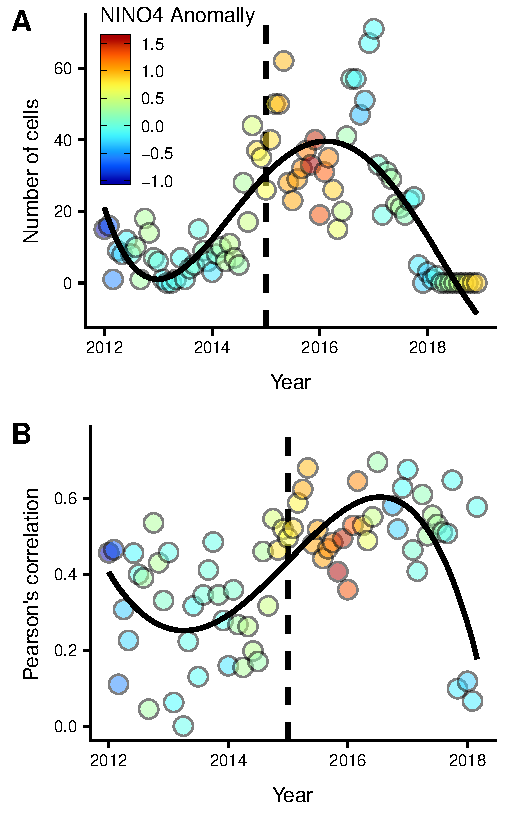
\includegraphics{img/KIR_sp_corr.pdf}
\caption{\label{fig:KIR_sp_corr}Number of cells that had displaced and non-displaced vessels (A) and spatial correlation in the presence-absence of each group per cell (B) for Kiribati's EEZ only. The solid lines represent the 4\textsuperscript{th} degree polynomial fit reported in \ref{tab:sp_corr}. Note that the late 2016 and early 2017 showed negative or neutral NINO4 anomalies, similar to those in the pre-PIPA period.}
\end{figure}

\begin{landscape}

\begin{table}[!htbp] \centering 
  \caption{\label{tab:main_DID}Difference-in-differences estimates for our 10 variables of interest: 1) Daily fishing hours, 2) Daily non-fishing at-sea hours, 3) Daily proportion of fishing hours to total at-sea hours, 4) Daily distance traveled, 5) Daily mean distance from port for fishing events, 6) Daily mean distance from shore for fishing events, 7) Monthly fishing hours spent in Kiribati waters, 8) Monthly fishing hours spent in PNA waters. Numbers in parentheses are heteroskedastic-robust standard errors.} 
  \label{} 
\footnotesize 
\begin{tabular}{@{\extracolsep{1pt}}lcccccccc} 
\\[-1.8ex]\hline 
\hline \\[-1.8ex] 
\\[-1.8ex] & (1) & (2) & (3) & (4) & (5) & (6) & (7) & (8)\\ 
\hline \\[-1.8ex] 
 Constant & 0.497$^{***}$ & 3.607$^{***}$ & 0.075$^{***}$ & 5.203$^{***}$ & 12.997$^{***}$ & 12.461$^{***}$ & 3.678$^{***}$ & 4.445$^{***}$ \\ 
  & (0.022) & (0.012) & (0.004) & (0.029) & (0.021) & (0.019) & (0.192) & (0.151) \\ 
  & & & & & & & & \\ 
 Post & 0.839$^{***}$ & $-$0.228$^{***}$ & 0.137$^{***}$ & 0.304$^{***}$ & 0.326$^{***}$ & 0.296$^{***}$ & 1.059$^{***}$ & 1.180$^{***}$ \\ 
  & (0.016) & (0.008) & (0.003) & (0.019) & (0.014) & (0.014) & (0.140) & (0.109) \\ 
  & & & & & & & & \\ 
 Treated & 0.136$^{***}$ & 0.014$^{**}$ & 0.015$^{***}$ & 0.400$^{***}$ & 0.223$^{***}$ & 0.116$^{***}$ & 0.534$^{***}$ & 0.149 \\ 
  & (0.013) & (0.007) & (0.002) & (0.020) & (0.016) & (0.016) & (0.148) & (0.118) \\ 
  & & & & & & & & \\ 
 Post $\times$ Treated & $-$0.244$^{***}$ & 0.013 & $-$0.034$^{***}$ & $-$0.483$^{***}$ & $-$0.281$^{***}$ & $-$0.155$^{***}$ & $-$0.565$^{***}$ & $-$0.399$^{***}$ \\ 
  & (0.019) & (0.009) & (0.003) & (0.022) & (0.017) & (0.017) & (0.161) & (0.127) \\ 
  & & & & & & & & \\ 
\hline \\[-1.8ex] 
Month FE & Yes & Yes & Yes & Yes & Yes & Yes & Yes & Yes \\ 
Flag FE & Yes & Yes & Yes & Yes & Yes & Yes & Yes & Yes \\ 
Observations & 83,052 & 83,052 & 83,051 & 64,387 & 32,055 & 32,055 & 1,814 & 2,588 \\ 
R$^{2}$ & 0.102 & 0.072 & 0.107 & 0.028 & 0.062 & 0.080 & 0.113 & 0.198 \\ 
\hline 
\hline \\[-1.8ex] 
\textit{Note:}  & \multicolumn{8}{r}{$^{*}$p$<$0.1; $^{**}$p$<$0.05; $^{***}$p$<$0.01} \\ 
\end{tabular} 
\end{table} 

\end{landscape}

\begin{figure}
\centering
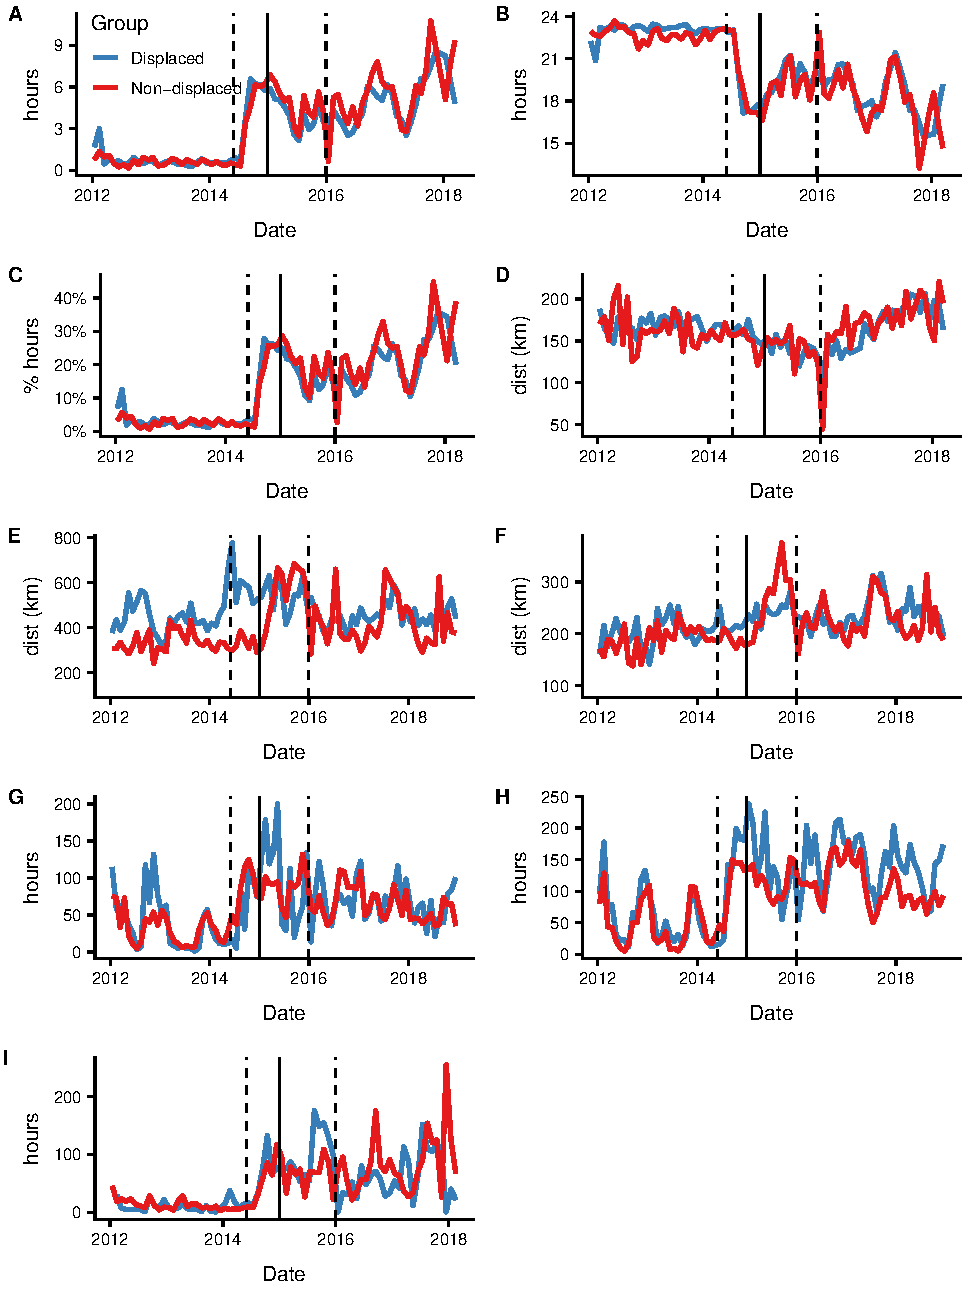
\includegraphics{img/all_panels.pdf}
\caption{\label{fig:all_panels}Time series showing monthly averages for our nine variables of interest: A) Fishing hours, B) Non-fishing hours at-sea, C) Proportion of fishing hours to total hours at-sea, D) Distance traveled, E) Mean distance from port for fishing events, F) Mean distance from shore for fishing events, G) Monthly hours spent in Kiribati waters, H) Monthly hours spent in PNA waters, I) Monthly hours spent on the high seas. Dashed vertical lines indicate the addition of new AIS satellites. Solid vertical line indicates the closure of PIPA.}
\end{figure}

\begin{figure}
\centering
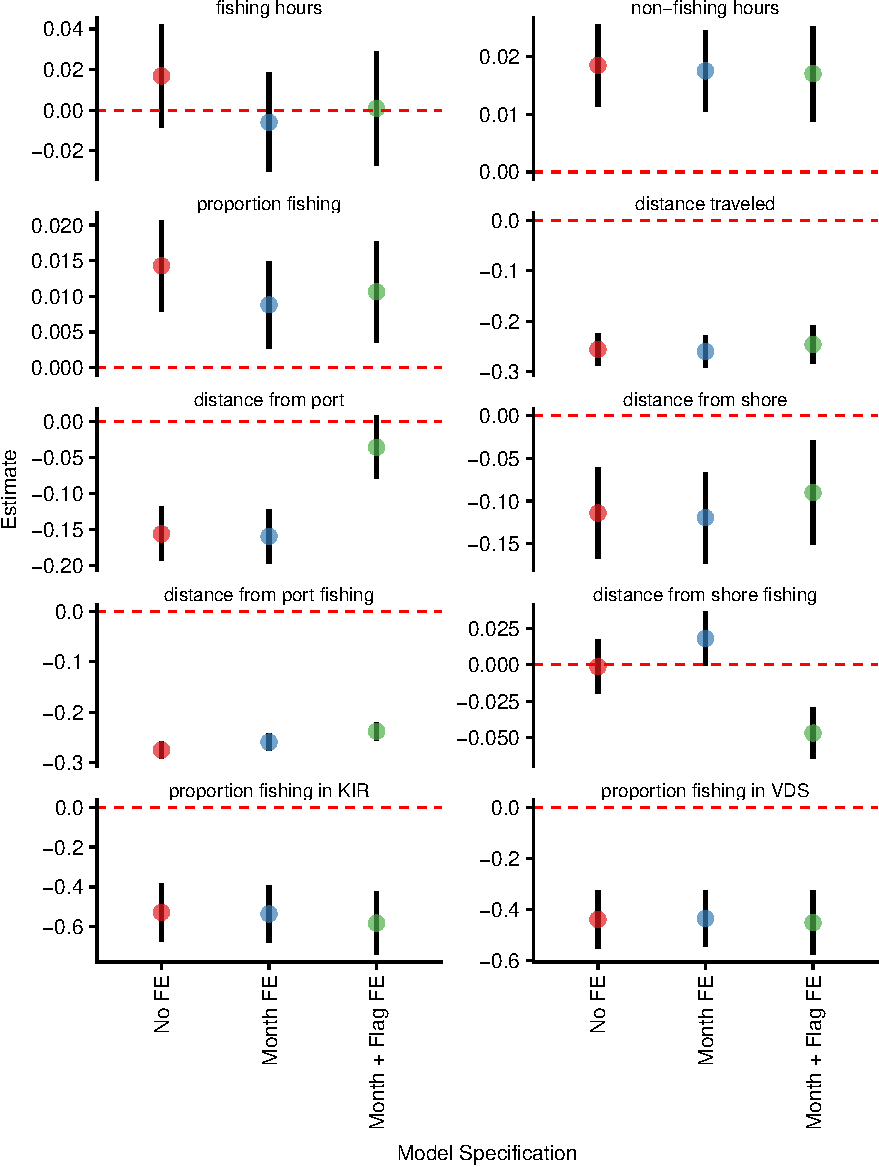
\includegraphics{img/other_specifications.pdf}
\caption{\label{fig:other_specifications}Alternative difference-in-differences estimates for our variables of interest using different model specifications. Table \ref{tab:main_DID} reports estimates for models with month and flag fixed effects, and NINO4 index (\emph{i.e.} green dots).}
\end{figure}

\begin{landscape}

\begin{table}[!htbp] \centering 
  \caption{\label{tab:main_DID}Difference-in-differences estimates for our 10 variables of interest: 1) Daily fishing hours, 2) Daily non-fishing at-sea hours, 3) Daily proportion of fishing hours to total at-sea hours, 4) Daily distance traveled, 5) Daily mean distance from port for fishing events, 6) Daily mean distance from shore for fishing events, 7) Monthly fishing hours spent in Kiribati waters, 8) Monthly fishing hours spent in PNA waters. Numbers in parentheses are heteroskedastic-robust standard errors.} 
  \label{} 
\footnotesize 
\begin{tabular}{@{\extracolsep{1pt}}lcccccccc} 
\\[-1.8ex]\hline 
\hline \\[-1.8ex] 
\\[-1.8ex] & (1) & (2) & (3) & (4) & (5) & (6) & (7) & (8)\\ 
\hline \\[-1.8ex] 
 Constant & 2.449$^{***}$ & 3.325$^{***}$ & 0.314$^{***}$ & 6.177$^{***}$ & 13.800$^{***}$ & 13.159$^{***}$ & 3.979$^{***}$ & 4.644$^{***}$ \\ 
  & (0.061) & (0.031) & (0.014) & (0.042) & (0.047) & (0.065) & (0.392) & (0.343) \\ 
  & & & & & & & & \\ 
 Post & 0.336$^{***}$ & $-$0.353$^{***}$ & 0.083$^{***}$ & 0.105$^{***}$ & 0.398$^{***}$ & 0.352$^{***}$ & 1.151$^{***}$ & 1.240$^{***}$ \\ 
  & (0.024) & (0.015) & (0.006) & (0.020) & (0.016) & (0.016) & (0.157) & (0.125) \\ 
  & & & & & & & & \\ 
 Treated & $-$0.085$^{***}$ & 0.060$^{***}$ & $-$0.028$^{***}$ & 0.259$^{***}$ & 0.259$^{***}$ & 0.163$^{***}$ & 0.435$^{***}$ & 0.082 \\ 
  & (0.027) & (0.014) & (0.007) & (0.020) & (0.018) & (0.018) & (0.163) & (0.133) \\ 
  & & & & & & & & \\ 
 Post $\times$ Treated & 0.036 & $-$0.052$^{***}$ & 0.019$^{***}$ & $-$0.296$^{***}$ & $-$0.342$^{***}$ & $-$0.199$^{***}$ & $-$0.481$^{***}$ & $-$0.335$^{**}$ \\ 
  & (0.028) & (0.017) & (0.007) & (0.024) & (0.020) & (0.019) & (0.179) & (0.142) \\ 
  & & & & & & & & \\ 
\hline \\[-1.8ex] 
Month FE & Yes & Yes & Yes & Yes & Yes & Yes & Yes & Yes \\ 
Flag FE & Yes & Yes & Yes & Yes & Yes & Yes & Yes & Yes \\ 
Observations & 25,004 & 51,724 & 25,004 & 52,767 & 25,004 & 25,004 & 1,399 & 2,010 \\ 
R$^{2}$ & 0.066 & 0.092 & 0.067 & 0.011 & 0.073 & 0.095 & 0.141 & 0.230 \\ 
\hline 
\hline \\[-1.8ex] 
\textit{Note:}  & \multicolumn{8}{r}{$^{*}$p$<$0.1; $^{**}$p$<$0.05; $^{***}$p$<$0.01} \\ 
\end{tabular} 
\end{table} 

\end{landscape}

\begin{landscape}

\begin{table}[!htbp] \centering 
  \caption{\label{tab:main_DID}Difference-in-differences estimates for our 10 variables of interest: 1) Daily fishing hours, 2) Daily non-fishing at-sea hours, 3) Daily proportion of fishing hours to total at-sea hours, 4) Daily distance traveled, 5) Daily mean distance from port for fishing events, 6) Daily mean distance from shore for fishing events, 7) Monthly fishing hours spent in Kiribati waters, 8) Monthly fishing hours spent in PNA waters. Numbers in parentheses are heteroskedastic-robust standard errors.} 
  \label{} 
\footnotesize 
\begin{tabular}{@{\extracolsep{1pt}}lcccccccc} 
\\[-1.8ex]\hline 
\hline \\[-1.8ex] 
\\[-1.8ex] & (1) & (2) & (3) & (4) & (5) & (6) & (7) & (8)\\ 
\hline \\[-1.8ex] 
 Constant & 2.637$^{***}$ & 3.247$^{***}$ & 0.404$^{***}$ & 5.016$^{***}$ & 13.177$^{***}$ & 12.684$^{***}$ & 3.259$^{***}$ & 4.096$^{***}$ \\ 
  & (0.042) & (0.021) & (0.011) & (0.044) & (0.028) & (0.025) & (0.270) & (0.206) \\ 
  & & & & & & & & \\ 
 Post & 0.283$^{***}$ & $-$0.443$^{***}$ & 0.048$^{***}$ & 0.628$^{***}$ & 0.164$^{***}$ & 0.077$^{***}$ & 1.347$^{***}$ & 1.586$^{***}$ \\ 
  & (0.039) & (0.021) & (0.011) & (0.044) & (0.024) & (0.022) & (0.234) & (0.188) \\ 
  & & & & & & & & \\ 
 Treated & $-$0.091$^{**}$ & $-$0.051$^{***}$ & $-$0.052$^{***}$ & 0.683$^{***}$ & 0.137$^{***}$ & $-$0.020 & 0.697$^{***}$ & 0.477$^{***}$ \\ 
  & (0.040) & (0.019) & (0.011) & (0.041) & (0.024) & (0.022) & (0.233) & (0.184) \\ 
  & & & & & & & & \\ 
 Post $\times$ Treated & 0.081$^{*}$ & 0.021 & 0.055$^{***}$ & $-$0.880$^{***}$ & $-$0.153$^{***}$ & 0.017 & $-$0.691$^{***}$ & $-$0.706$^{***}$ \\ 
  & (0.042) & (0.023) & (0.011) & (0.046) & (0.027) & (0.024) & (0.251) & (0.202) \\ 
  & & & & & & & & \\ 
\hline \\[-1.8ex] 
Month FE & Yes & Yes & Yes & Yes & Yes & Yes & Yes & Yes \\ 
Flag FE & Yes & Yes & Yes & Yes & Yes & Yes & Yes & Yes \\ 
Observations & 19,971 & 42,555 & 19,971 & 43,068 & 19,971 & 19,971 & 1,207 & 1,696 \\ 
R$^{2}$ & 0.064 & 0.097 & 0.066 & 0.032 & 0.059 & 0.071 & 0.133 & 0.217 \\ 
\hline 
\hline \\[-1.8ex] 
\textit{Note:}  & \multicolumn{8}{r}{$^{*}$p$<$0.1; $^{**}$p$<$0.05; $^{***}$p$<$0.01} \\ 
\end{tabular} 
\end{table} 

\end{landscape}

\begin{landscape}

\begin{table}[H] \centering 
  \caption{\label{tab:DID_without_USA_TWN}Difference-in-differences estimates for our 9 variables of interest after excluding US and Tawianese vessels. 1) Daily fishing hours, 2) Daily non-fishing at-sea hours, 3) Daily proportion of fishing hours to total at-sea hours, 4) Daily distance traveled, 5) Daily mean distance from port for fishing events, 6) Daily mean distance from shore for fishing events, 7) Monthly fishing hours spent in Kiribati waters, 8) Monthly fishing hours spent in PNA waters, and 9) Monthly fishing hours in the high seas. Numbers in parentheses are heteroskedastic-robust standard errors.} 
  \label{} 
\footnotesize 
\begin{tabular}{@{\extracolsep{1pt}}lccccccccc} 
\\[-1.8ex]\hline 
\hline \\[-1.8ex] 
\\[-1.8ex] & (1) & (2) & (3) & (4) & (5) & (6) & (7) & (8) & (9)\\ 
\hline \\[-1.8ex] 
 Constant & 0.536$^{***}$ & 3.600$^{***}$ & 0.082$^{***}$ & 4.506$^{***}$ & 13.002$^{***}$ & 12.438$^{***}$ & 3.850$^{***}$ & 4.719$^{***}$ & 2.420$^{***}$ \\ 
  & (0.023) & (0.012) & (0.004) & (0.043) & (0.022) & (0.020) & (0.209) & (0.158) & (0.419) \\ 
  & & & & & & & & & \\ 
 Post & 0.796$^{***}$ & $-$0.217$^{***}$ & 0.130$^{***}$ & 0.021 & 0.290$^{***}$ & 0.291$^{***}$ & 0.870$^{***}$ & 0.894$^{***}$ & 0.732$^{**}$ \\ 
  & (0.019) & (0.010) & (0.003) & (0.035) & (0.016) & (0.016) & (0.156) & (0.121) & (0.291) \\ 
  & & & & & & & & & \\ 
 Displaced & 0.142$^{***}$ & 0.016$^{**}$ & 0.015$^{***}$ & 0.341$^{***}$ & 0.227$^{***}$ & 0.127$^{***}$ & 0.490$^{***}$ & $-$0.017 & $-$0.296 \\ 
  & (0.013) & (0.007) & (0.002) & (0.031) & (0.018) & (0.017) & (0.163) & (0.126) & (0.239) \\ 
  & & & & & & & & & \\ 
 NINO4 & $-$0.001 & $-$0.001 & 0.001 & $-$0.383$^{***}$ & 0.189$^{***}$ & 0.082$^{***}$ & 0.325$^{***}$ & 0.171$^{***}$ & 0.441$^{***}$ \\ 
  & (0.011) & (0.006) & (0.002) & (0.019) & (0.009) & (0.008) & (0.075) & (0.063) & (0.122) \\ 
  & & & & & & & & & \\ 
 Post $\times$ Displaced & $-$0.212$^{***}$ & $-$0.002 & $-$0.029$^{***}$ & $-$0.158$^{***}$ & $-$0.328$^{***}$ & $-$0.184$^{***}$ & $-$0.533$^{***}$ & $-$0.225 & 0.339 \\ 
  & (0.021) & (0.010) & (0.004) & (0.039) & (0.019) & (0.018) & (0.175) & (0.138) & (0.291) \\ 
  & & & & & & & & & \\ 
\hline \\[-1.8ex] 
Month FE & Yes & Yes & Yes & Yes & Yes & Yes & Yes & Yes & Yes \\ 
Flag FE & Yes & Yes & Yes & Yes & Yes & Yes & Yes & Yes & Yes \\ 
Observations & 73,717 & 73,717 & 73,716 & 73,778 & 26,920 & 26,920 & 1,546 & 2,236 & 660 \\ 
R$^{2}$ & 0.095 & 0.072 & 0.102 & 0.021 & 0.077 & 0.094 & 0.111 & 0.169 & 0.256 \\ 
\hline 
\hline \\[-1.8ex] 
\textit{Note:}  & \multicolumn{9}{r}{$^{*}$p$<$0.1; $^{**}$p$<$0.05; $^{***}$p$<$0.01} \\ 
\end{tabular} 
\end{table} 

\end{landscape}

\begin{figure}
\centering
	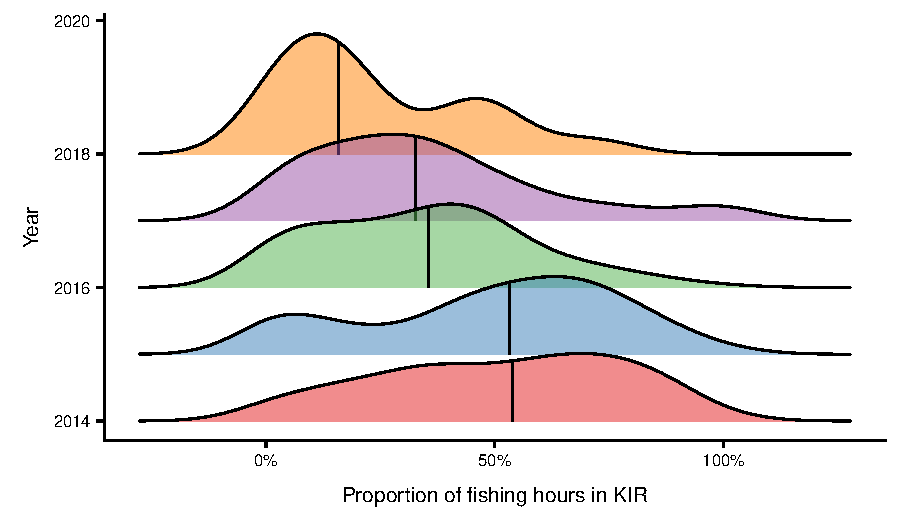
\includegraphics{img/hist_kir_fishing.pdf}
	\caption{\label{fig:hist_kir_fishing}Ridgeplot for the density of the \% of total fishing hours that take place within Kiribati EEZ waters by year for displaced vessels where the unit of observation is an individual vessel.}	
\end{figure}

\begin{figure}
\centering
	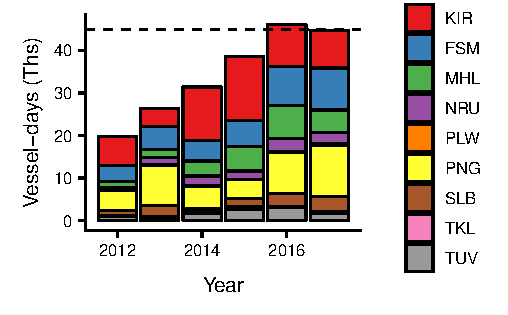
\includegraphics{img/all_PS_VDS_cty_year.pdf}
	\caption{\label{fig:all_PS_VDS_cty_year}Annual vessel-days for all PNA countries, by country.}
\end{figure}

\begin{figure}
\centering
	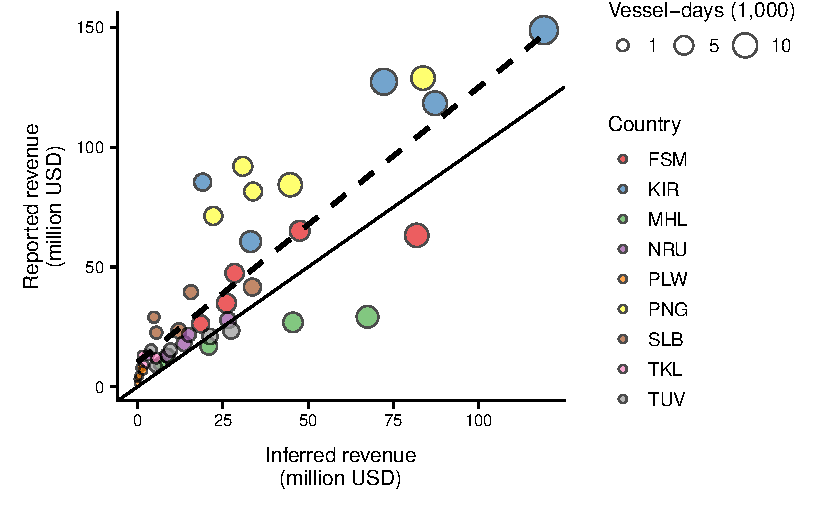
\includegraphics{img/revenue_FFA_GFW_linear.pdf}
	\caption{\label{fig:revenue_FFA_GFW_linear}Inferred revenues vs. reported revenues. The dashed line represents line of best fit, and the solid line represents a 1:1 line.}
\end{figure}

\begin{figure}
\centering
	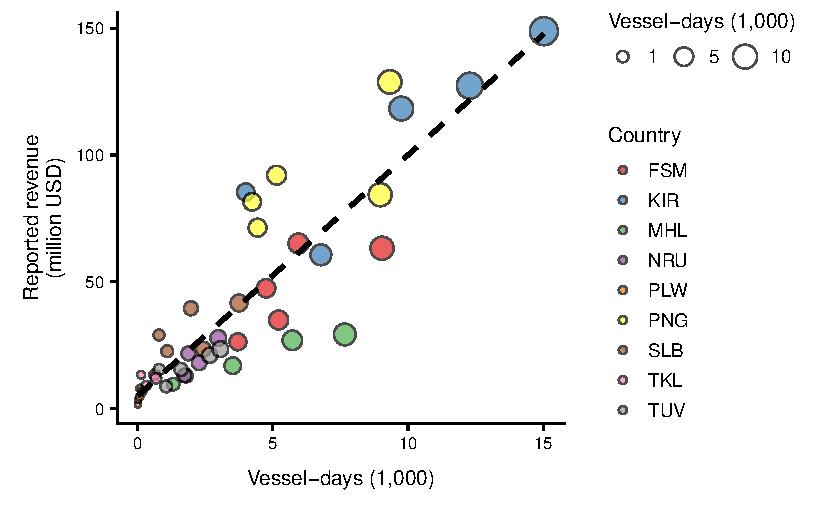
\includegraphics{img/revenue_FFA_effort_GFW.pdf}
	\caption{\label{fig:revenue_FFA_effort_GFW}Observed fishing effort vs. reported revenues. The dashed line represents line of best fit.}
\end{figure}

\begin{figure}
\centering
	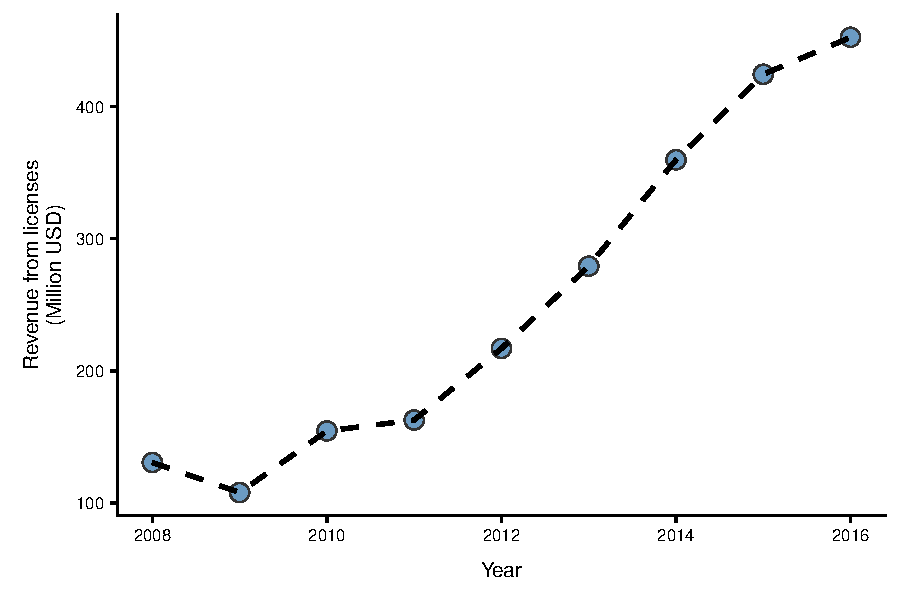
\includegraphics{img/total_PNA_revenues.pdf}
	\caption{\label{fig:total_PNA_revenues}Total revenues for all PNA countries combined.}
\end{figure}

\begin{figure}
\centering
	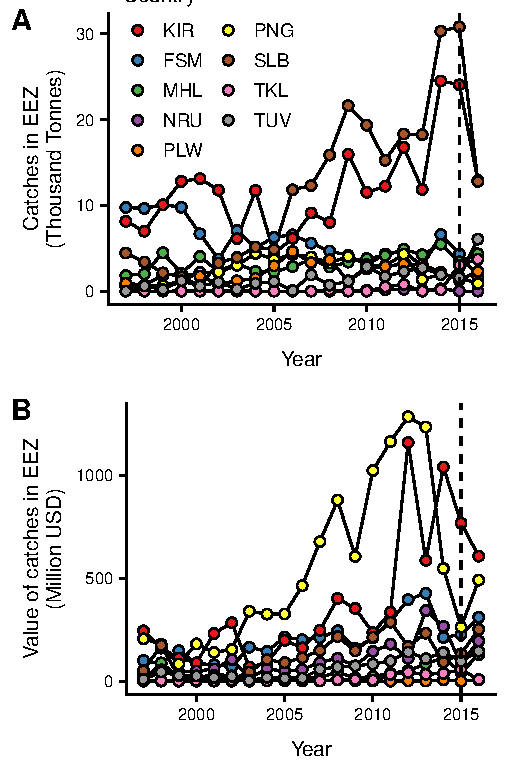
\includegraphics{img/catches.pdf}
	\caption{\label{fig:catches}Financial indicators for PNA countries. A) Total annual purse seine catch by EEZ and, B) Total annual value of purse seine catch by EEZ. Vertical dashed line in both plots denotes implementation of PIPA.}
\end{figure}

\begin{figure}
\centering
	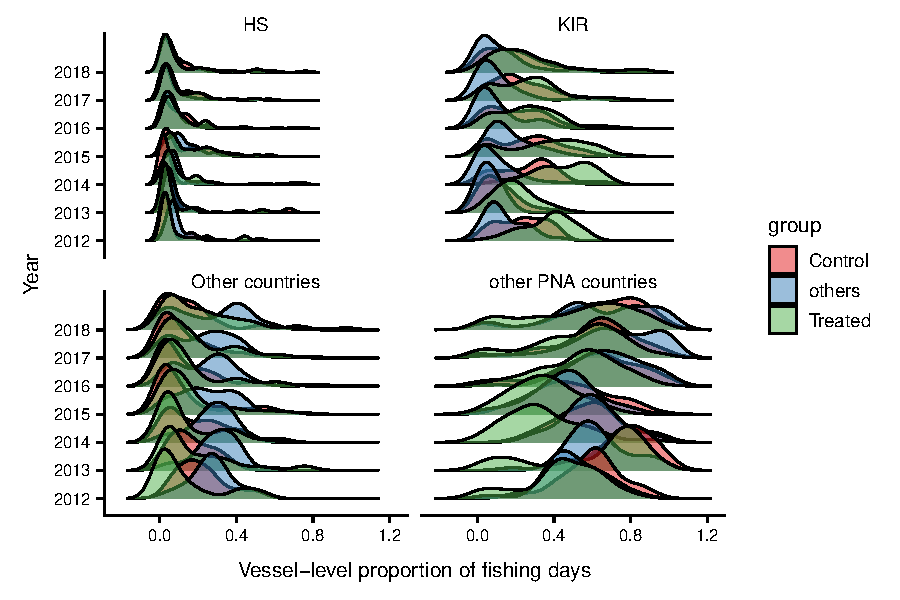
\includegraphics{img/yearly_distribution_prop_fishing_by_region.pdf}
	\caption{\label{fig:yearly_distribution_prop_fishing_by_region}Ridgeplot for the density of the \% of total fishing hours that take place in each region for all vessels}	
\end{figure}

\clearpage

\begin{figure}
\centering
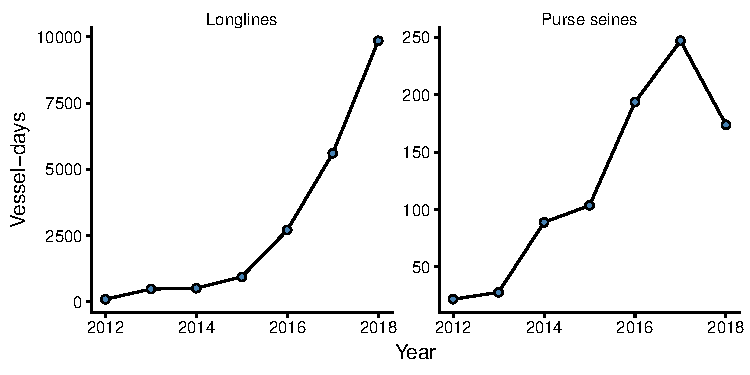
\includegraphics{img/PLW_GFW_ts.pdf}
\caption{\label{fig:PLW_GFW_ts}Timeseries of longline and purse seine fishing effort in Palaw.}
\end{figure}

\end{document}
